\documentclass[a4paper, 11pt]{article}
\setlength{\topmargin}{0in}
\setlength{\textheight}{8in}
\setlength{\oddsidemargin}{.1in}
\setlength{\textwidth}{6in}

\usepackage{multirow}
\usepackage{float}
\usepackage{array}
\usepackage[document]{ragged2e}
\usepackage{comment} 
\usepackage{subcaption}
\usepackage{amssymb,amsmath}
\usepackage[font={small,it}]{caption}

\usepackage{datetime}
\usepackage{tgbonum}

\newdateformat{mydate}{\monthname[\THEMONTH] \THEYEAR}

\newcolumntype{L}{>{\centering\arraybackslash}m{3cm}}

\newcommand{\tab}[1]{\hspace{.2\textwidth}\rlap{#1}}
\usepackage{graphicx}
\graphicspath{{images/}}

\begin{document}


\LARGE\title{User Modelling in Search for People with Autism}

\LARGE\author{Author: \textbf{Esha Massand}, Supervisor: \textbf{Keith Mannock}\\
\\
MSc Computer Science\\Department of Computer Science and Information Systems\\Birkbeck College, University of London\\\\\\Project report submitted in partial fulfilment of the requirement for the \\MSc in Computer Science\date{\mydate\today}
\\\
}

\normalsize


\maketitle


\section*{Abstract}
\begin{justify}
This project report presents my research and the development of a prototype web application to assist users with Autism when they search the web. The system has modelled user interactions with the search process into a user profile for this category of users, integrating insights from the core features of autism into the model. The system is integrated with an infra-red, motion controlled, user interface component to assist users with Autism during search. The project provides insights into how search can be improved for users with Autism.\\
\end{justify}
\begin{verbatim}






\end{verbatim}

\begin{justify}
This project is substantially the result of my own work, expressed in my own words, except where explicitly indicated in the text. I give my permission for it to be submitted to a Plagiarism Detection Service. This proposal may be freely copied and distributed provided the source is explicitly acknowledged.
\end{justify}



\begin{center}
word count (project text only) : 8443 words
\end{center}

\clearpage
\tableofcontents
\clearpage

\section*{Abbreviations}
\begin{tabular}{l l }
API & Application Programming Interface\\
AQ & Autism Quotient\\
ASD & Autism Spectrum Disorder\\
DSM & Diagnostic and Statistical Manual\\
GCS & Google Custom Search\\
HCI & Human Computer Interaction\\
HTTP & Hypertext Transfer Protocol\\
IDE & Integrated Development Environment\\
KWIC & Key Word In Context\\
LEAP & LEAP Motion Controller\\
REST & Representational state transfer\\
RIFT & Oculus Rift Virtual Reality Head Mounted Display\\
TDD & Test Driven Development\\
UI & User Interface\\
UX & User Experience\\
VR & Virtual Reality\\
\end{tabular}

\section*{Definitions}

\begin{tabular}{l p{11cm}  }
Autism & Autism is amongst the most common neuro-developmental condition and it is currently estimated that 1/68 children meet criteria for Autism Spectrum \cite{CDC}. Autism is five times more common amongst boys than girls (1/42 boys, and 1/189 girls). According to the Diagnostic and Statistical Manual (2013), Autism is characterised by persistent and early deficits in reciprocal social interaction and repetitive behaviours. Individuals vary from high functioning to low functioning (along a spectrum), with behaviours emerging around 2 to 3 years of age.\\


Stereotyped User Model & Stereotyped user models infer characteristics about a user from data gathered from other users within that distinct subset. They can be built quickly using clusters of characteristics of groups of individuals. 

\end{tabular}
\clearpage

\section*{Search Engine Measures}
\newcommand{\cfplus}{\mathbin{\genfrac{}{}{0pt}{}{}{+}}}

\subsection*{Precision}
The field of information retrieval defines precision as the fraction of retrieved documents that are relevant to the query. 

\begin{equation*}
Precision
=\frac{|(relevant\ documents) \land (retrieved\ documents)|}{|(retrieved\ documents)|}
\end{equation*}

\subsection*{Recall}
The field of information retrieval defines recall as the fraction of relevant documents that are retrieved by the search query. 

\begin{equation*}
Recall
=\frac{|(relevant\ documents) \land (retrieved\ documents)|}{|(relevant\ documents)|}
\end{equation*}
\clearpage

\section{Introduction}\label{intro}

\begin{comment}
Contains a brief outline of the topic as a whole
Then state the aim and objectives of the project
What was the purpose of the project and what did it set out to investigate?
At the end of the introduction, provide a road map for the
remainder of the report
\end{comment}

This project report presents my aim to research and develop a prototype web application for people with Autism when they search the web. This project will combine interactive, motion recognition hardware with search to improve the UI (user interface) of search for individuals with Autism. 

\subsection {Background Research}\label{background} 

According to the Diagnostic and Statistical Manual \cite{CDC}, Autism is characterised by persistent and early deficits in reciprocal social interaction. Autism is the most common neurodevelopmental condition (1/68 children meet criteria for Autism Spectrum \cite{CDC}). It is well known that interaction with computers is prominent in this group, and that individuals with Autism are more engaged when using technology that is receptive and interactive (e.g., games, responsive consoles, motion controlled devices) compared to technology that is not \cite{motioncontrollerforautism}. 

\vspace{5mm}
Research has shown that people with Autism are less context-sensitive \cite{mottron}. Generally speaking, individuals with Autism prefer, and are more likely to engage in an item-specific, or detailed processing style. There is good reason to postulate then, that web-search queries are formed very differently to the typical population, more likely consisting of single-order associations. In addition to a detailed, item-specific processing style, individuals with Autism are also less likely to engage in a contextual processing style. For example in a search for `Guitar', a contextual style of processing would imply an awareness that the word is related to `Piano', but also that both words are hierarchically related to `Instrument'. 

\vspace{5mm}
Working memory is the memory system that assists with the transient holding and processing of information for updating, learning and comprehension. In day to day life, a major factor determining the effectiveness of working-memory and the quality of information that an individual can recall (e.g., enter into the web-search), is the number of cues that are available at the time. For example, if presented with a list of 50 items to remember, you are more likely to remember that I presented `Zebra' if I tell you that I presented an animal than if no cue of `animal' was given. This type of `cued' recall can be used to bolster recall of information, and is a technique that will be applied in the current project to enable individuals with Autism to formulate better search queries in their browser. \\

\subsection{The Problems with Current Web-Search}\label{What should search offer people with Autism}

The Internet is one of the largest resources of information. Search engines allow users to collate hundreds of links on a single topic, using only a few words or phrases. The typical user sorts the returned results into `relevant' or `irrelevant' categories, flexibly shifting (mentally) between one result and the next, to determine the relevance of each page returned by the search engine. Search allows the user to assimilate the information on the page into their knowledge and is an important learning tool. For people with Autism, the requirement is no different, however, I argue that for individuals with Autism, current search is not adequate. A large body of research has shown that `mental shifts' are a known area of weakness for people with Autism \cite{disengagement}. The information is therefore harder to assimilate or learn, and judging the relevance of each document `on the fly', and speedily, becomes near impossible. One successful Psychological technique to increase the assimilation of information for individuals with Autism is to present it in clearer, smaller amounts \cite{AdultsWithAutism}. This technique avoids overwhelming individuals, and although less information is presented as a whole, whatever is presented to the user becomes `digestible' and ultimately, the information as a whole becomes more understandable.  \\

\vspace{5mm}

Search queries usually fall into one of three broad categories \cite{seo}.  `Do' queries which characterise transactions between the user and the search engine, for example when the user wants to do something such as \textit{buy a plane ticket}, \textit{listen to a song} or, \textit{download a screensaver}. `Know' type queries, which are informational in nature, usually covering a broad topic, for example, the \textit{name of a band} or \textit{restaurant in London}, \textit{trucks}, or \textit{Colorado}. The third broad category is `Go' type queries, which are navigational in nature, for example, searching for a particular home page on the web, \textit{YouTube} or \textit{American Airlines}. There are also many stages to the search process \cite{seo}. After identifying the information need, the user must formulate a search query. The user must browse through results once the query has been entered into a search engine. The whole process can be repeated if the user is not satisfied. 

\begin{enumerate}
\item{Experience the need for an answer,
solution, or piece of information.}
\item{Formulate that need in a string of words and phrases, also known as `the query'.}
\item{Enter the query into a search engine.}
\item{Browse through the results for a match.}
\item{Click on a result}
\item{Scan for a solution, or a link to that solution.}
\item{If unsatisfied, return to the search results and browse for another link or ...}
\item{Perform a new search with refinements to the query}
\label{search flows}
\end {enumerate}

\subsection{Current Project}
This project report presents a prototype browser-based application to assist users with Autism when they search the web. The application is hereafter referred to as Jellibeans\footnote{Jellibeans are a rainbow of colours, different sizes and shades, and the name represents the difference in style of processing of individuals with ASD.}. Jellibeans utilises gesture and hand movement data recorded using the Leap Motion Controller (LEAP) to enable an interactive search in the web browser. 

\vspace{5mm}
One aim of the current project was to build a tool that synthesised three leading search engines. The tool can be used to present the top results of search queries to ensure the best possible results were retrieved and presented to the user. The first stage was to therefore build the combination search engine and test the results on a user group with Autism. The goal of the research was to understand if the synthesis of the search engines enhanced search experience (in other words were users happy with the combination search), or, whether the results introduced redundancies or oddities in the results.\\

\vspace{5mm}
In programmatic terms, Jellibeans implements a research-guided user model in search. The developer for the current project has extensive research experience from working with individuals with Autism, and will apply these insights into the development of the Jellibeans. The development of this user model consisted of iterations of the `research, development, test, evaluate' lifecycle. I conducted research surveys to identify differences in user queries and analysed search behaviour patterns from people with and without Autism. Using these data I built a set of features into search, to guide the user through forming a more complete search query. Development and evaluation included the implementation and testing of the features, and further implementation and revision of the software to enhance the search process and the precision of the search engine for the users' intended search query. 

\vspace{5mm}
Jellibeans integrates a motion controlled user interface (UI) using the LEAP motion controller. The interface is very dynamic as opposed to static, which can hold users' attention for long periods of time. In the past, users with Autism have struggled to maintain their attention to sift through the large number of search results. In line with the attention difficulties individuals with Autism face, Jellibeans has been designed to reduce the amount of text on the search results page, presenting only 3 results per page, instead of the default 10. 

\subsection{Parametric Search Design for Web Applications}

Search engines like Google apply strong reduction techniques to navigation of the web. For example, one common way this reduction pattern is implemented is by assuming the behaviour of the current user is similar to the behaviour of other users in similar situations. The principle applied by Google is to `make it easy' for the user \cite{googleTerms}, by assuming that users form search queries similarly, and returning similar results to those users. This is often seen in other recommendation engines also, e.g., Amazon. 

\vspace{5mm}
As we have seen in the introduction, users with Autism behave in different ways to typical users when navigating search. Users with Autism do not use the same key phrases when looking for documents with several attributes, i.e., queries that would be best formulated using several iterations of search, or multiple search parameters. This leads to an ineffective search; one that requires users to sift through results which are in large-part irrelevant, and a bad user experience.  

\vspace{5mm}
Parametric search queries allow users to specify parameters for their search in an increasingly logical and structured way. As an example, consider the experience of searching for flights to a particular holiday destination. This requires high cognitive `load' (remembering and manipulating arrival, departure, destination, timings, airlines, seat preferences etc.) so searches are often structured using fixed options (see Figure~\ref{exped}).

\begin{figure}[H]
\begin{center}
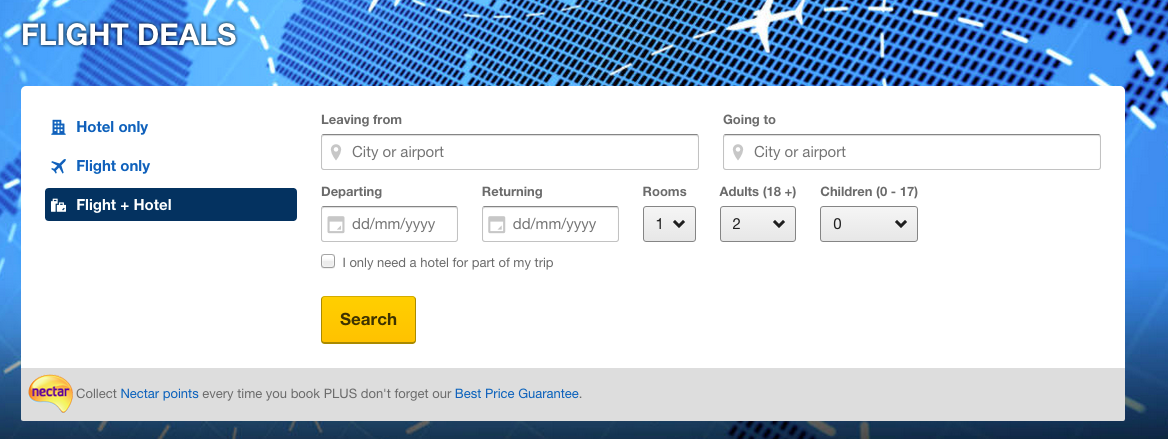
\includegraphics[scale=0.27]{expedia}
\caption{Expedia Parametric Search Example}
\label{exped}
\end{center}
\end{figure}

For typical users, parametric search is more structured, and in some circumstances seems more natural than a free keyword search. It makes search queries easier to formulate in situations where there is a high cognitive load.  We can apply this idea to web search for people with Autism, by asking them to enter criteria that can be applied to subgroups of search queries. Parametric search can assist the user with capturing the search parameters that are useful for a query, but it does not ultimately reduce the number of search results returned; the possibility of a large result set is most definitely true. So, although this tackles one aim of Jellibeans, further refinement of the search results would also be necessary.

\subsection{Motion controllers}
Individuals with Autism have poor attention \cite{attention}. The static 2-dimensional interface of many current search engines is unlikely to maintain adequate (sustained) interest levels. Individuals (and especially teenagers) with Autism spend a substantial amount of their time using computers, web, portable or console devices \cite{Shane and Albert}, as they find these more stimulating and attention-grabbing. For these individuals, computer-based technologies provide a stable, consistent learning environment that can be customized \cite{moore}. Furthermore, motion recognition devices can be programmed to make consistent responses to environmental triggers. These controlled and interactive environments have shown promise for improving social communication skills and reducing repetitive behaviours \cite{gameshealth}. For the current project a motion-controlled learning environment will be bolstered to improve attention within search for people with autism. 

\begin{figure}[H]
\begin{center}
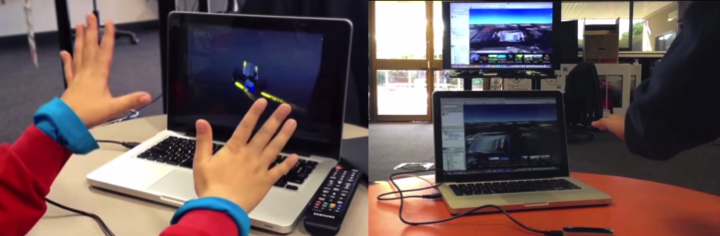
\includegraphics[scale=0.47]{vision}
\caption{UI component for the project \cite{leap}.}
\label{vision}
\end{center}
\end{figure}

\subsection {Aims for Jellibeans}
Jellibeans is a prototype search tool that assists users with Autism search and navigate the web. As search can be compartmentalised into `Do', `Know' and `Go' type queries, it provides a natural way to tackle the issue of simplifying the search process for people with Autism. Users first identify the type of search they would like to carry out. Then Jellibeans better phrases a question to guide the user through their informational demand. Each stage of the search flow process is better tailored towards providing a concrete and unambiguous experience for the user with Autism, and reducing the amount of text on the page. 

\vspace{5mm}
When using Jellibeans, users are assisted through the process of formulating a search query, much like a parametric search engine form (for example when you buy a car, you fill out many criteria which must be simultaneously searched for). Concretely phrased questions are aided by suggestions that appear laterally on the page. The user can add these suggestions into their search query without the need to type them in, just by using natural hand movements, tracked by the LEAP motion controller. The UI component makes the experience of searching the web more interactive and receptive for user input. The suggestions also serve as cues for the user, and to simplify the search process for them. 

\vspace{5mm}
The implementation of a parametric-like search means the process of forming a query is more tightly defined and predictable for the user compared to the current systems for web search. The size of the result-set is also reduced, and adapted towards users with Autism. 

\vspace{5mm}
Each of these features were tested in one-on-one interviews and a group of users with Autism\footnote{Autism diagnostic status was determined using the Autism Quotient, which strictly speaking is not a diagnostic assessment tool. However the measure has a 79\% sensitivity to Autism if the user scores above 32 on the measure.}. The prototype was integrated into the web browser and within a motion-controlled environment. The prototype was modified accordingly in line with the outcome of several stages of user research. An agile methodology was used to build the final prototype using static HTML. The static website prototype can be found at esha.mseth.co. \\

\vspace{5mm}
Using Jellibeans, users can complete a screening tool for Autism and save their score to a database so that they can log in and out of Jellibeans at their convenience. Jellibeans will remember their Autism score the next time they sign in.

\vspace{5mm}
The final product is presented at the end of this report, and is written using php, JavaScript, HTML and CSS (using BootStrap). The dynamic website has a greater degree of functionality and promise for future updating. The dynamic website was created once the `quick and dirty' prototype was completed. The final prototype can be found at jellibeans.mseth.co.

\vspace{5mm}
The core features of Jellibeans are:

\begin{enumerate}
\item {A web-based search tool, that uses a \textit{stereotyped}\footnote{Stereotyped user models infer characteristics about a user from data gathered from other users within that distinct subset.} user model of Autism to filter search results. The features of the model were determined following analyses of survey responses gathered from 7 individuals with Autism or a high occurrence of autism-like symptoms (above a score of 30 on the Autism Quotient). The survey was administered online using a web-based survey engine \cite{surveymonkey}, and focused on identifying the differences in user search query generation for people with autism. The individual participants also took part in a one on one interview session and focus group at the end of project.}

\item {Jellibeans implements a parametric-like search to gather a number of search keywords from the user. Jellibeans returns small snippets on the results page to a maximum of 3 search results per page (the result page is not verbally-overloaded).}

\item {Jellibeans prioritises results which have first-order semantic relations to the query words. Jellibeans employs a boolean `AND' between each search word searched for, so that results are more likely first order semantic relations to the searched query.}

\item {Jellibeans uses a data store to saves the user's Autism score for the next time they sign in. The user's score and the search queries that were formed using Jellibeans, were used to evaluate the search tool. The datastore was implemented using MySQL.}

\item {Jellibeans implements within a motion controlled UI which uses the LEAP controller. This makes search more interactive and receptive for users. The LEAP also works to maintain the attention of the user.}

\end{enumerate}

\subsection{Challenges}
There are several expected challenges for the current project. One such challenge concerns the very nature of trying to develop a tool for individuals with Autism, knowing that there is a large variability in the phenotype (or presentation) of the condition. Trying to address the clinical features of Autism across the entire spectrum is no mean feat. The sample selected for the current study were \textit{verbal} adults with high functioning Autism, or Asperger Syndrome. 

\vspace{5mm} 
Another challenge relates to gathering feedback on Jellibeans. I conducted focus groups and interviews which required lot of verbal communication. This is always a challenge when working with individuals who are known to have difficulties with communication.

\vspace{5mm}
More of a technical challenge concered the reliance on open source APIs which were not regularly maintained. For resources that were incomplete, I implemented the tools myself, or, I searched for alternative ways to achieve that goal. The same applied for the open source libraries and packages that I used for the current project.

\vspace{5mm}
To complete the aims for the current project within the time frame was chanllenging given that most of the project used novel technologies for the developer. These included building the user model within a dynamic website, learning php, HTML, CSS, JavaScript and JQuery, and, integrating the motion controlled user interface within that framework. 

\vspace{5mm}
Conducting surveys, interviews and a focus group to gather feedback on the tool, and to implement this feedback into a revised prototype for Jellibeans was a time consuming task. Often this required that I worked around participant schedules. Two participants out of the 7 were unavailable during the user feedack stage of the study, and so these particpants were excluded from any subsequent analyses.

\section{Project Specification and Design} 

The following requirements were proposed for Jellibeans web application. 

\begin{figure}[H]
\begin{center}
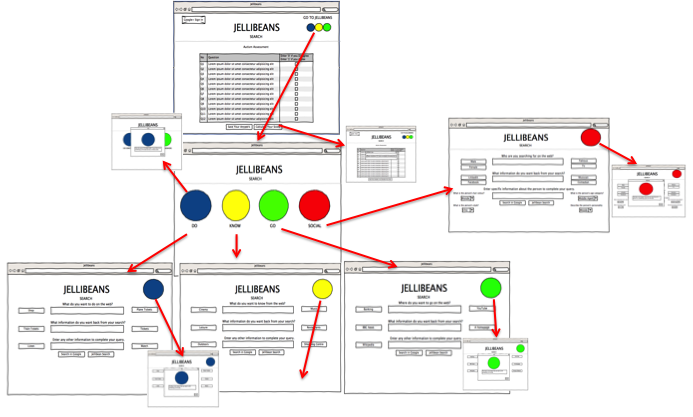
\includegraphics[scale=0.65]{JellibeanUserFlow.png}
\end{center}
\caption{Wireframe Sketches for Jellibeans User Flow. A prototype version of Jellibeans using static html pages can be found at http://esha.mseth.co. A dynamic and near-production version of Jellibeans using routes rather than static html, which is fully LEAP motion controller-enabled can be found at jellibeans.mseth.co. }
\label{JBeanUserFlow}
\end{figure}

\vspace{5mm}
Jellibeans implemented a combination search web application that synthesised the results from three of the largest and most popular engines; Google, Bing and Yahoo \cite{adam}.

\vspace{5mm}

Jellibeans integrates with Google+, to allow the user to sign in and have their profile picture and name displayed, enhancing the feel of a personalised search engine (see Figure~\ref{googlesignin}).

\begin{figure}[H]
\begin{center}
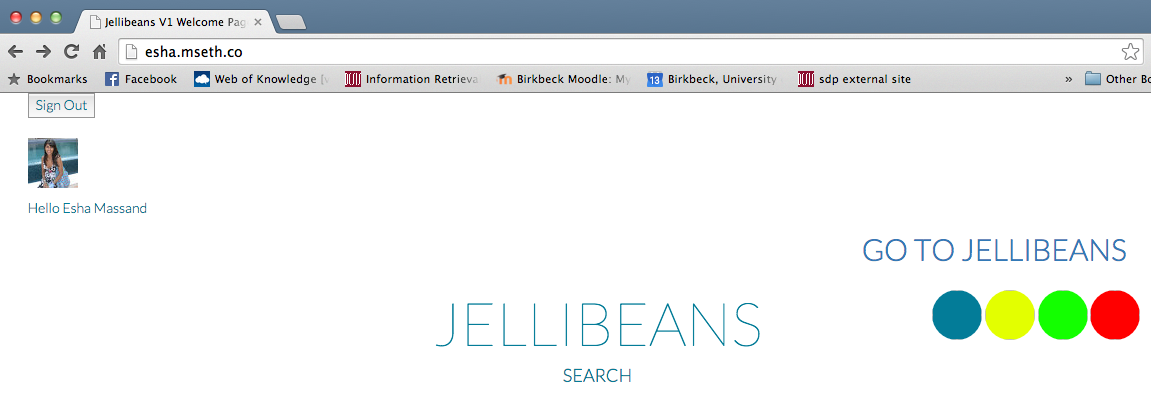
\includegraphics[scale=0.25]{helloEsha}
\end{center}
\caption{Using the Google+ API Allowed the User to Sign In and Retrieve User Name and Profile Picture.}
\label{googlesignin}
\end{figure}

Jellibeans employs a parametric-like search, including \textit{suggestions} to guide the user towards forming succinct and accurate search queries (see Figure~\ref{JBeanUserFlow}). Once signed in, the user can fill out the Autism Quotient and get feedback regarding their autism symptomology. The Autism Quotient \cite{Baron Cohen et al} is a Psychological assessment and validated screening tool for autism spectrum disorders. Users can also save their responses for each question to a local file for their reference.

\begin{figure}[H]
\begin{center}
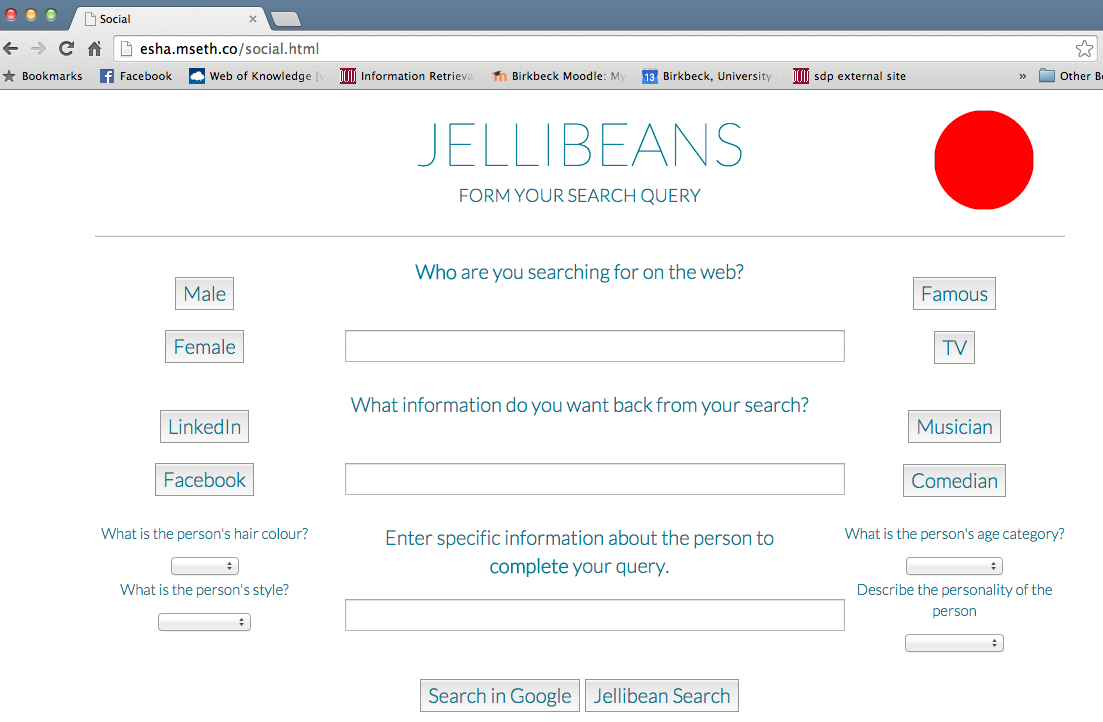
\includegraphics[scale=0.25]{SocialPage}
\end{center}
\caption{An example page from Jellibeans: the Social Query page.}
\label{SocialPage}
\end{figure}


Jellibeans web application is integrated with a motion controlled UI, the LEAP controller (see Figure~\ref{UserMakingQuery}) giving the application a receptive and interactive user interface.

\begin{figure}[H]
\begin{center}
\includegraphics[scale=0.15]{UserMakingQuery}
\caption{User Forming A Jellibean Search Query with LEAP Using Both Hands.}
\label{UserMakingQuery}
\end{center}
\end{figure}

Jellibeans prioritises and displays the three highest precision search results for users. Recall of the search engine is sacrificed in line with the demands of the user model, to have less textual information on the page.

\vspace{5mm}
Jellibeans reduces the amount of text on the webpage by having results display on a modal (a hovering display panel on the page) which can be easily closed, and reopened to display results (see Figure~\ref{resultsModal}). Due to the nature of parametric search, strict boolean operators used in Jellibeans, and the reduced number of search results displayed, the results from Jellibeans are a direct semantic relation to the search query. 

\begin{figure}[H]
\begin{center}
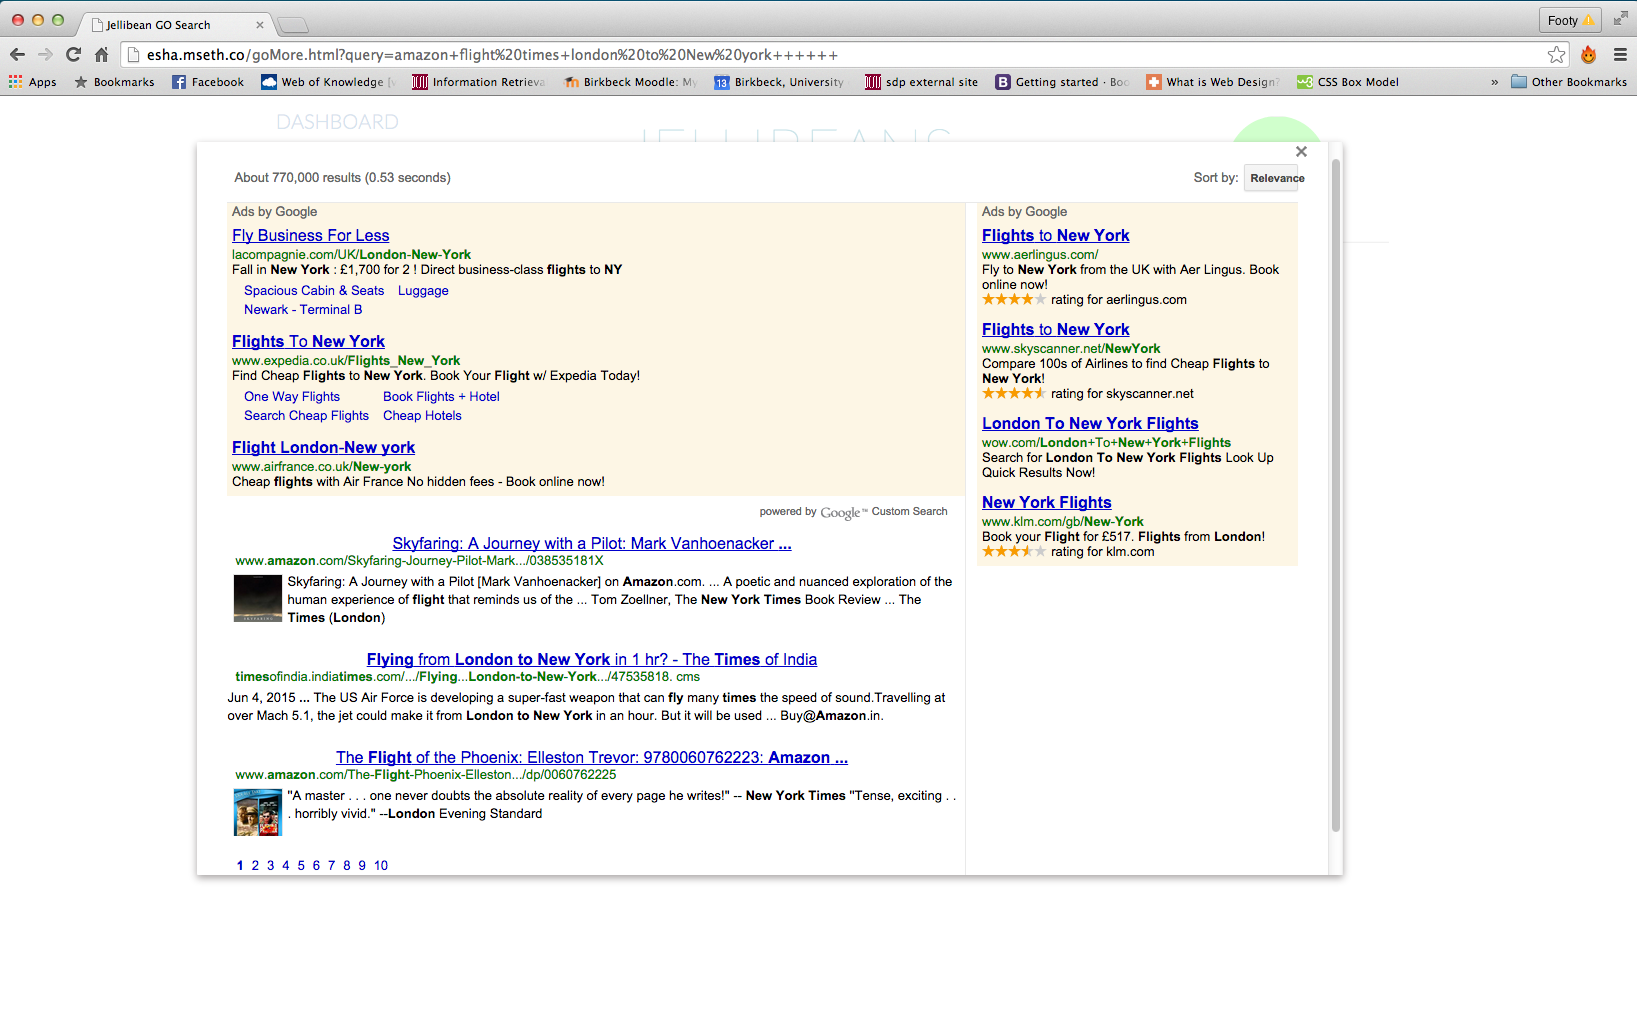
\includegraphics[scale=0.25]{ResultsModal}
\end{center}
\caption{Top 3 results are presented back to users in a modal to reduce information on the page. The modal can easily be closed and reopened.}
\label{resultsModal}
\end{figure}

\begin{comment}

\section{Product Specification}
The Functional Requirements of Jellibeans are: 

\begin{itemize}
\item{Java Applet for the Combination Search Engine (Java).}
\item{Rendering the Application to the Web Browser (HTML, CSS, BootStrap, php).}
\subitem{Integration with Google+ API (JavaScript and JQuery).}
\subitem{Integration with Google Custom Search API (JavaScript).}
\item{LEAP Motion Controller (LEAP SDK and LeapStrap).}

\end{itemize}

\end{comment}

\section{System and Software Architecture}

\subsection{Architecture of the System: 3-tier Architecture}
A client-server software architecture was used for Jellibeans. The user interface and motion controller formed the presentation layer, the logic layer was made up of the JavaScript code used to implement the custom search, and storage of data in the data store were maintained as three distinct modules. The advantages of this type of design is that it allows each of the tiers to be modified, upgraded or replaced independently of one another. For example, if Jellibeans were to be implemented with another motion controller (e.g. the Oculus VR Rift), it would only impact the Presentation tier (see Figure~\ref{ntier}).
\begin{figure}[H]
\begin{center}
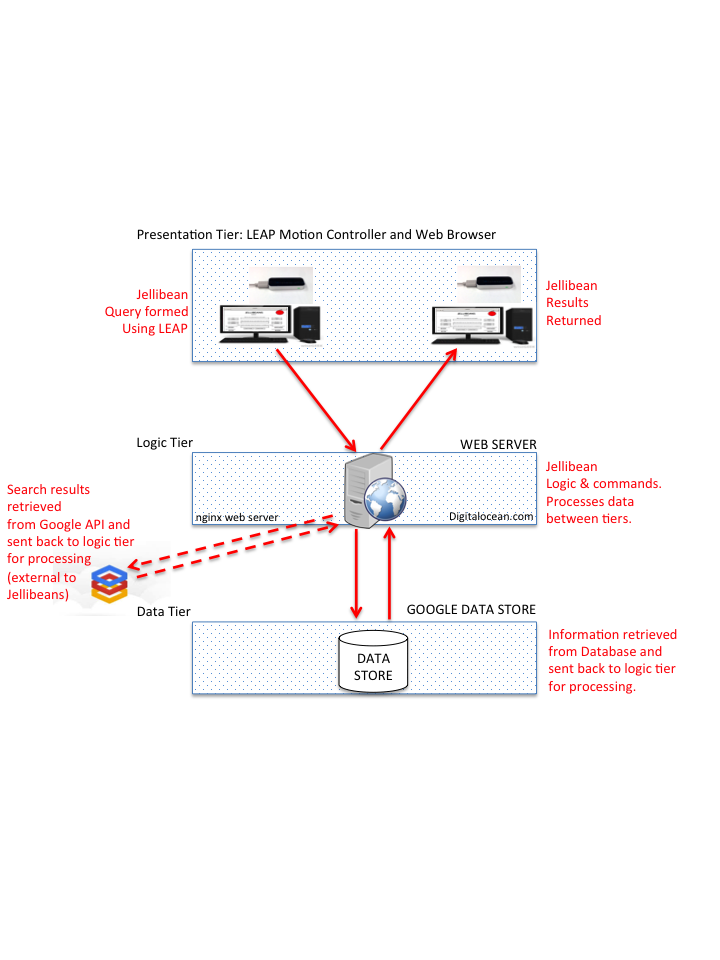
\includegraphics[scale=0.65]{ntier}
\caption{3-tier architecture implementation}
\label{ntier}
\end{center}
\end{figure}

To see a list of the API's, development languages used and their justifications, see Appendix~\ref{implementation}. The APIs and languages are listed in the context they were used below.\\

\vspace{5mm}

\begin{itemize}
\item{Presentation Module\\
The presentation module consists of:}

\subitem{Jellibean Web Application: Rendering the web application to the browser (HTML, CSS PHP and Bootstrap).}

\subitem{Rendering a Parametric-Like Search in the browser: The user is asked specific questions to break down their search query into smaller manageable terms, i.e., into `Do', `Know', `Go', or `Social' queries, and then into direct search terms. This reduces the ambiguity individuals with Autism face when forming a search query. The web application provides suggestions or cues for users. Once the search terms are entered by the user, they are sent to the logic module to form the search query string, and then onto the data store to retrieve the results which are subsequently rendered onto the screen for the user (HTML, CSS, php and Bootstrap).}

\subitem{Google+ Integration: Jellibeans integrates with Google+ API to retrive and render user profile data. This enhances the feel of a personalised search engine. Once signed in, users complete a diagnostic assessment of Autism (the Autism Quotient \cite{Baron Cohen et al}). The user's entries are sent to the logic module to be calculated. A user can also save a copy of their diagnostic information to a local file on their computer (JQuery, JavaScript and Google+ API).}

\subitem{The user's AQ score is saved to the database once the score is calculated. The score is fetched from the database whenever the user logs in. A unique identification number assures that the user data is never overwritten or duplicated.}

\subitem{LEAP UI Component: Jellibeans is a LEAP enabled website, and has a Motion Controlled UI in the web browser. The motion controller provides an interactive search experience, and maintains the user's full attention during search (LEAP SDK and LeapStrap).}

\item{Logic Module\\
At the logic layer, Jellibeans works to build user search queries from the elements on the web page. The parameters are entered by the user when they form their search query at the presentation layer. The Builder Design pattern was used to build a complete search query, and submit these to the Data Store so that the result pages could be returned to the user. \\
The logic module enables:}

\subitem{Logic to produce a combination search engine that synthesises the search results from Google, Bing and Yahoo. The aim of this feature is to increase recall of the search engine (Java).}

\subitem{Logic to integrate with the Google+ API (JavaScript and Google+ API).}

\subitem{Calculation of the users' AQ Score using the questionnaire entries that are entered at the presentation layer. The request is sent to the database (MySQL). The score is returned to the presentation layer after calculation (JavaScript).}

\subitem{Logic to formulate the user's search query, given their entries at the presentation layer (JavaScript).}

\subitem{Logic to send the query to the Google Data Store, and, to retrieve the search results to render them to the presentation layer (JavaScript and Google Custom Search API).}

\subitem{Logic to prioritise the three highest ranking search results and to reduce the text and verbal information on the page (in line with the aims of Jellibean Search), (JavaScript and Google Custom Search API).} 

\subitem{The logic layer communicates with the Google Data Store layer to retrieve the search results for the user.}

\item{Data Store Module}
\subitem{Jellibeans works with a database to store and retrieve the users Autism score each time the user signs in (MySQL). }
\subitem{Jellibeans works with the Google Custom Search engine to retrieve the (indexed) documents from the Google data store. The documents that are retrieved match the participants' search query string after processing at the logic module level. }
\end{itemize}

\section{Software Design Pattern}
I will now describe the design pattern that guided the software development process. The final Jellibeans prototype uses the model-view-controller (MVC) software design pattern. There are three components to the MVC pattern (see Figure ~\ref{laravelMVC}). 

\begin{figure}[H]
\begin{center}
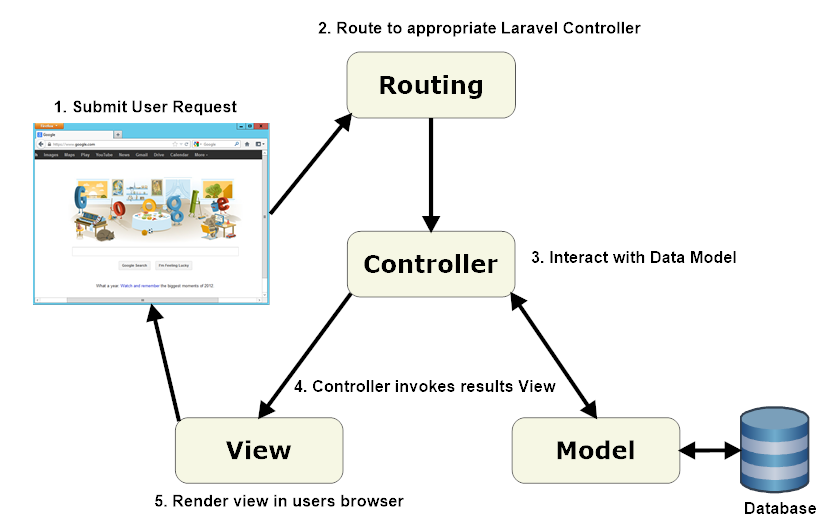
\includegraphics[scale=0.45]{laravelMVC}
\end{center}
\caption{Application Model-View-Controller pattern as described by the Laravel framework\cite{laravel}.}
\label{laravelMVC}
\end{figure}

For Jellibeans this results in the following components and classes:

\begin{itemize}
\item{The \textbf{Model}- is the domain or real world entity that the software is built around. The model in this case is the User.}
\item{The \textbf{View}- is the visual representation of the user, given a context. So, in this case it is the resulting markup that the php framework (Laravel) renders to the users browser (i.e., the html code). The view generates the user interface, and is accessible via the user(model). The view doesn't handle the data that comes in (although users input the data into the view that is presented). There are 6 views of the system.}
\subitem{\tab{index.php renders the homepage}}
\subitem{\tab{search.php renders the Search screen}}
\subitem{\tab{do.php renders the Do search page}}
\subitem{\tab{know.php renders the Know search page}}
\subitem{\tab{go.php renders the Go search page}}
\subitem{\tab{social.php renders the Social search page}}
\subitem{\tab{result.php renders the Results page}}
\item{The \textbf{Controller}- Coordinators provide links between the view and the model. Coordinators are responsible for input-processing and determining the behaviour of Jellibeans, such as rendering a new screen. Controller.php is an abstract class that all other controllers extend see Figure~\ref{controller}. Jellibeans has the following Controllers:}
\subitem{PagesController.php controls the page behaviour when a user clicks on the navigation buttons, for example, return the user back to the homepage.}
\subitem{RegistrationController.php controls the model's storing and registering of the user and user credentials.}
\subitem{SearchController.php controls the behaviour of which search to carry out given the view.}
\subitem{SessionsController.php controls the behaviour of the view depending on whether the user is logged in or logged out. For example, if the user is logged out it will display the register and login buttons on the html page. If the user is logged in, it will return the logout button. It also }
\subitem{UserController.php verifies the CRUD (Create, Read, Update and Delete) actions form the resource.}
\end{itemize}

\begin{figure}[H]
\begin{center}
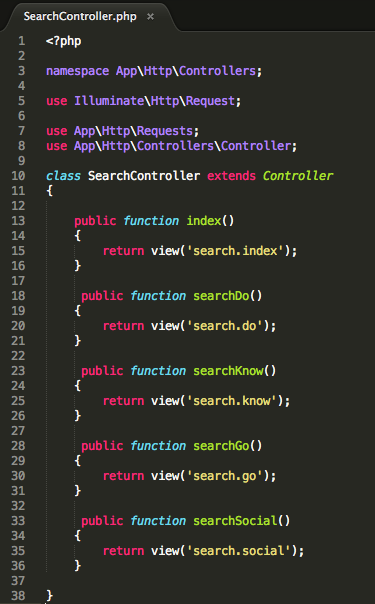
\includegraphics[scale=0.55]{controllers}
\caption{Example of a Controller Class (the SearchController class) which return views of the system dependent on user behaviour.}
\label{controller}
\end{center}
\end{figure}


\begin{itemize}
\item{The \textbf{Routes} - decompose the configuration of which action of that controller should receive the request.} 
\subitem{Application Routes were set up which listed the URIs that Jellibeans should respond to, and the Controller to call when that URI is requested (see Figure~\ref{routes}).}
\end{itemize}

\begin{figure}[H]
\begin{center}
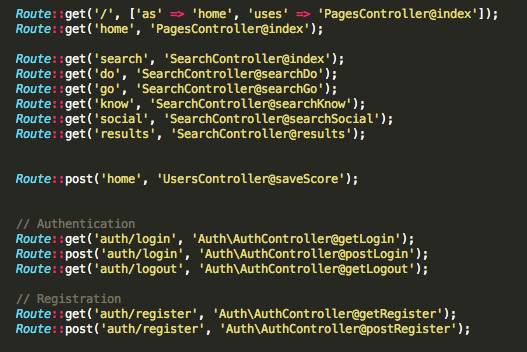
\includegraphics[scale=0.65]{routes}
\caption{Example class of how Routes were defined.}
\label{routes}
\end{center}
\end{figure}

Then present a class diagram which has 
\begin{comment}
Views-> resources/views/search
do.php
go.php
know
social
results
index

-------

Controllers -> app/http/controllers 
implemented to control the flow of the pages
controller.php abstract which all other controllers extend

PagesController -  returns the user back to the homepage.

RegistrationController - the Registration controller returns views for storing and registering the user.

SearchController - controlls the flow html pages that are related to search, including the homepage, do, know, go, social, and the search results page.

SessionsController - controls the flow between pages if the user is logged in versus logged out. For example, if the user is logged out it will display the register and login buttons on the html page. If the user is logged in, it will return the logout button.

UsersController - CRUD Create, Read, Update and Delete form the resource.

-------

Model - User -> app/user
database table to be used by the model
\end{comment}

\vspace{5mm}
A high level class diagram of the system can be seen in Appendix~\ref{jBeanClassDiagram}.

\vspace{5mm}
A use case diagram of the system can be seen in Appendix~\ref{JBeanUseCaseA}.

\begin{comment}
 to the JavaScript methods in the relevant class (dependent upon the user's search behaviours), parsed into the correct format, before a POST request is then made to the Jellibeans Custom Search Engine to process the request.
\item{Chain of responsibility Pattern.}\\
Because there are many behaviours that the user can perform before their query string is formulated and ready to be posted to the search engine, the software also makes use of the Chain of responsibility pattern where at each stage the user's query is passed along a chain, with added functionality and methods depending on what the behaviour of the user was.
\item{Adapter Pattern.}\\
I accessed the user's Google+ profile data (name and profile picture) and presented these on the Jellibeans homepage. I then used the Adapter design pattern to build my own functionality onto the existing profile. For example, to present the user's Autism Quotient score, and to guide the user through forming their search query. 

The software design patterns that were chosen to implement the logic layer, and software architecture (3 tier) to implement Jellibeans work together to reduce coupling between the interface (web browswer and motion controller), logic (classes and the query), and data store layers. 
\end{comment}


\begin{comment}
\subsection*{TODO}
API's and Development Tools\\
Describe the technologies used in the project, why they where
chosen and what were the other options:\\
Tools and programming languages\\
\end{comment}

\section{Implementation}
The prototype version of Jellibeans is hosted at esha.mseth.co. This prototype was used for user testing, to quickly and cheaply develop and test the system. The prototype version of Jellibeans used static web pages which allowed the prototype to be quickly tested and finalised.

\vspace{5mm}
Jellibeans was finalised into a dynamic website and is hosted at jellibeans.mseth.so. The advantages of a dynamic website are that it is much more functional, no need to edit individual html pages, and no code repetition. 

\vspace{5mm}
The next section of the report describes how each module of work was completed.

\subsection{Combination Search Engine: Google, Yahoo and Bing.} 
To implement the combination search engine I used three API's provided by Google, Bing and Yahoo, namely, the Google Custom Search API, Yahoo BOSS Java API and Bing Search API. 

\vspace{5mm}
To get started with the Google Custom Search API, I created a project called \textit{Jellibeans} in the Google Developers Console, and an OAuth 2.0 Client ID. I obtained a Consumer Key and Secret to use the API, and used these in the application code to access the Google Custom Search Engine (see Figure~\ref{JBeanAppletGoogleCustomSearch1}). 

\begin{figure}[H]
\begin{center}
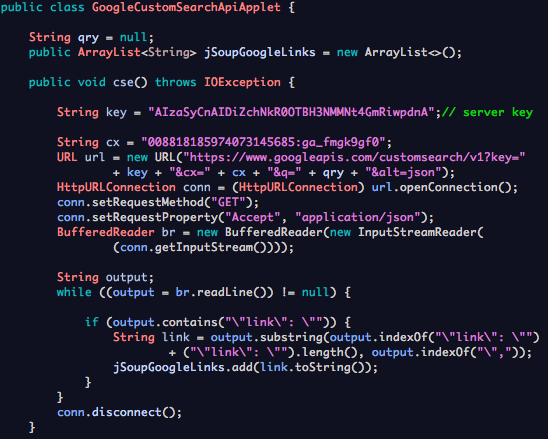
\includegraphics[scale=0.7]{JBeanAppletGoogleCustomSearch}
\end{center}

\caption{Jellibean Applet Combination Search Engine}
\label{JBeanAppletGoogleCustomSearch1}
\end{figure}

Following that I also registered my JavaScript origins within the console to access the Google+ API, and redirected URIs so that once users Sign-In using their Google+ login credentials they will be redirected to Jellibeans (or http://esha.mseth.co). This was done because I wanted users to be able to sign in and access their google profile from Jellibeans (see Figure~\ref{GoogleSignInPage}), giving the user the feel of a more personalised search experience. 

\begin{figure}[H]
\begin{center}
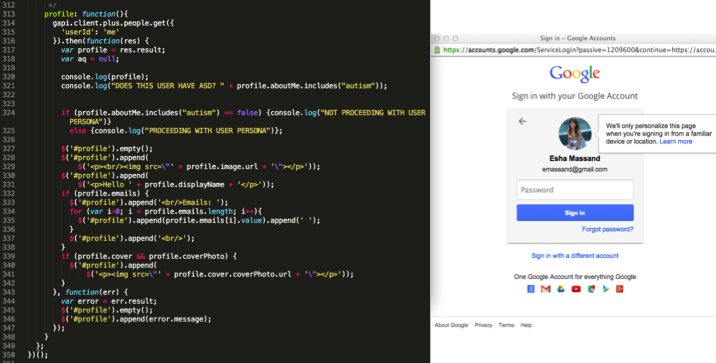
\includegraphics[scale=0.65]{aboutme}
\end{center}
\caption{Google+ Integration Code and Sign In Pop-Up (JQuery).}
\label{GoogleSignInPage}
\end{figure}

Following a similar protocol for Yahoo and Bing Search API's, I created projects in the Yahoo Developers Network, and Microsoft Azure Marketplace, and purchased an API Consumer Keys and Secrets (for use with the APIs). 

\subsubsection{Web Scraping}
As Bing and Yahoo Search API's were not opensource, I explored the efficacy of web scraping using the JSoup API. With the JSoup API I was able to retrieve the search results in line with the goal for the first aim of project, using a different href filter for each search engine. Web-Scraping is however, against Google policies (see section 5.3 of Appendix~\ref{GoogleToS1} for Google Terms of Service). 

\vspace{5mm}
I used the Jsoup API \cite{jsoup}, which is a Java-written API for HTML. The library provides methods to conveniently extract data using the DOM (Data Object Model) and CSS (Cascading Style Sheet) methods. 

\vspace{5mm}
The combined Google, Yahoo and Bing results were integrated these into a Java Applet that runs in Eclipse Luna IDE (see Figure~\ref{AppletFig}). The program ran so that the user could enter a search query and the results would be presneted back to them for inspection. The top 10 links, from each search engine were presented to users. Results were ranked prior to presentation, such that result 1 from Google was followed by result 1 from Yahoo, and that was followed by result 1 from Bing. Then results 2 from Google, Yahoo and Bing were presented and so on, until the 30 links were produced (top 10 links for a search from each search engine), in ranked order from the three search engines. 

\begin{figure}[H]
\begin{center}
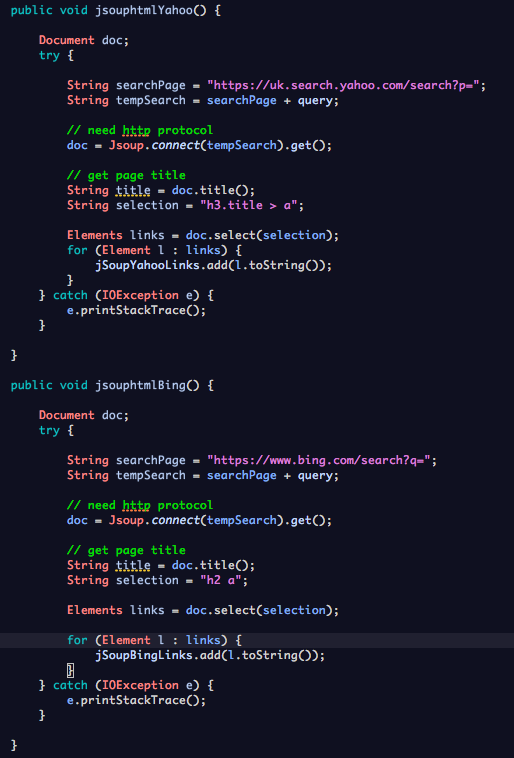
\includegraphics[scale=0.60]{htmlParsers}
\end{center}
\caption{JSoup HTML Parser for Yahoo and Bing Search Engines.}
\label{GoogleSignInPage}
\end{figure}

\begin{figure}[H]
\begin{center}
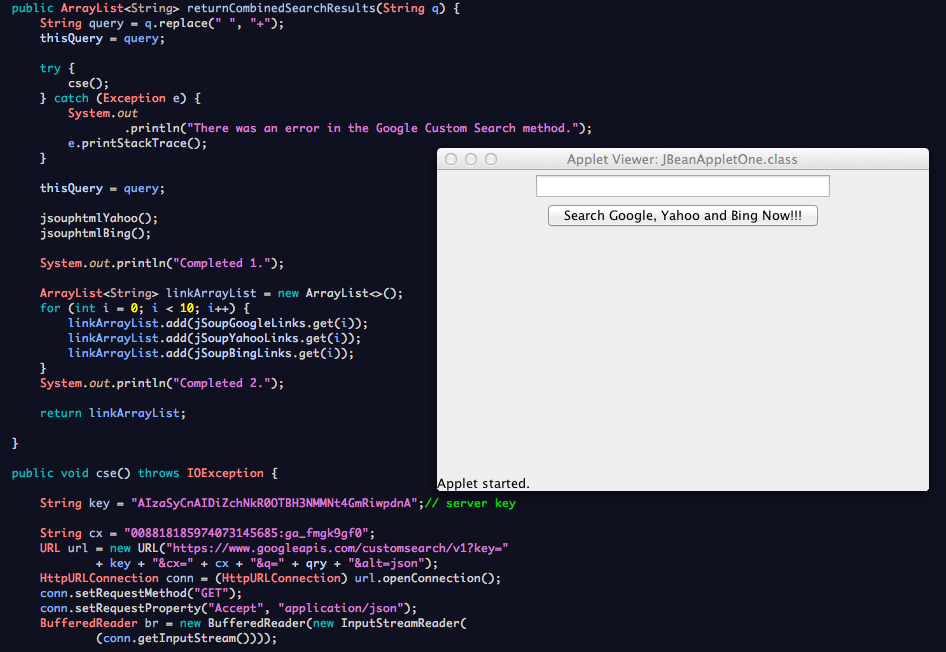
\includegraphics[scale=0.47]{Applet}
\end{center}
\caption{Yahoo and Bing Results Integrated with Google Custom Search to Produce the Complete Query Results.}
\label{AppletFig}
\end{figure}

\begin{comment}
\begin{figure}[H]
\centering
\begin{subfigure}{.55\textwidth}
  \centering
  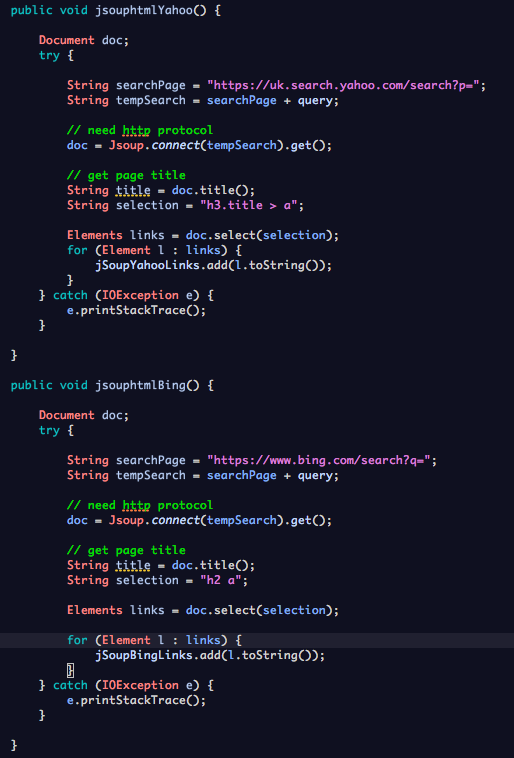
\includegraphics[width=.75\linewidth]{htmlParsers}
  \caption{JSoup HTML Parser for Yahoo and Bing Search Engines.}
\end{subfigure}%
\begin{subfigure}{.60\textwidth}
  \centering
  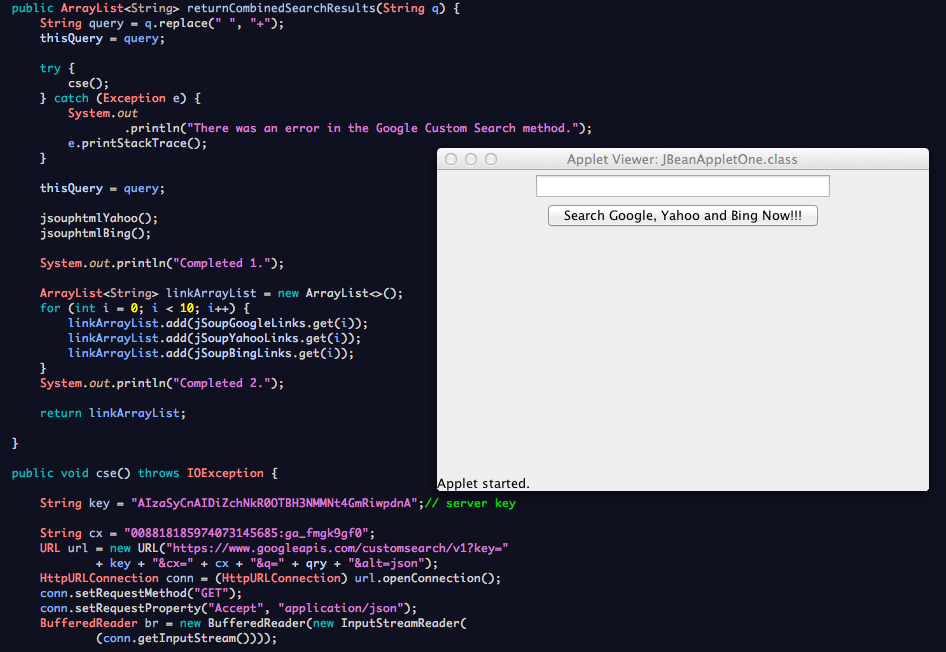
\includegraphics[width=.75\linewidth]{Applet}
  \caption{Integration with Google Custom Search to Produce the Complete Query Results.}
\end{subfigure}
\caption{(a) JSoup HTML Parsers for Yahoo and Bing. (b) JSoup HTML Parsers working with Google Custom Search API in Java Applet for User Testing.}
\label{AppletFig}
\end{figure}
\end{comment}





\subsection{Building a User Model of Autism.}
To identify the features of the user model to build, I ran a study to collect example search queries on a set of informational needs from 37 participants. The participants were asked to give examples of search queries they would use to, for example, identify the name of a song they had heard (given the lyrics), or the name of a breed of a dog they had seen (given a picture of the dog). There were in total 10 search queries; the study was distributed widely via Surveymonkey.com \cite{surveymonkey} and can be seen in the Appendix ~\ref{AppendixA}. All participants were also asked to complete the Autism Spectrum Quotient 50-item questionnaire see Appendix ~\ref{AQ}. The participants responses are analysed and reported back to surveymonkey.


\vspace{5mm}
Participants were divided into two groups; low AQ scorers (scores below 30), and high AQ scorers (scores equal to and above 30). There were 30 low AQ scorers and 7 high AQ scorers. 


\subsubsection{Differences in Search Queries Between Users With and Without Autistic-like traits.}
I conducted a qualitative analysis on the search query strings from both low and high AQ scorers.

\vspace{5mm}
To confirm the results from the user testing of Core Feature 1, participants were asked to indicate which search engine they commonly use, and in both groups, Google was the prefered search engine by far, with all participants reporting that they used Google as a first choice. No one in the current sample used Yahoo or Bing.

\vspace{5mm} 
The low AQ scorer responses were analysed together to establish a baseline answer. This was generated using a frequency criterion of 40\% i.e., if 12 out of 30 respondents or more generated the same portion of a query string given an informational need, it was included in the model below. If two responses were equally as common, both are reported in the model. Data was discarded when a response indicated that the participant would do an image search, as this was not the aim of the survey. The results from the frequency analysis are presented below.

\begin{enumerate}
\item{You hear a song on the radio with the lyrics, `Look at your children', and you want to download it. What would you type into search on your favourite search engine to find out what song it was?\\\textit{Look at your children song}. \\\textit{Look at your children lyrics}.}
\item{You've lost touch with an old school friend (you went to St. Mary's School). What key words/queries would you use to find them?\\\textit{St. Mary's School Year of X}.}
\item{How would you identify what this is using a search engine (pretend you don't know what it is called). What key words/queries would you use?\\\textit{Star shaped brown plant}.}
\item{How would you find out the name of this famous person using a search engine? What key words/queries would you use?\\\textit{Brown hair famous young women}.}
\item{How would you identify what breed this animal is using a search engine? What key words/queries would you use?\\\textit{Small dog fluffy breed}.}
\item{Your friend and you can't agree on how Thandie Newton pronounces her first name. How would you resolve this using a search engine?\\\textit{Thandie Newton pronunciation}.}
\item{What would you search for to identify this pattern's name, and which country it originates from?\\\textit{Repeating square maze pattern border}.}
\item{How would you search for delay's relating to your (imminent) flight to Paris?\\\textit{Flight number, Paris, airport, flight time}.}
\end{enumerate}

There was a lot more variation in the responses gathered from the group with Autistic-like traits. The responses can be seen in Appendix~\ref{asdresponses}. The following observations were made for the users in the high AQ group:
\begin{enumerate}
\item{There were an increased number of incompletely-formed queries. In the high AQ group, participants were more likely to miss off words in the query string. For example, when analysing the results from query 1 above, 2 out of 7 respondents in the high AQ group did not put `lyrics' or `song' in the search query when searching for the lyrics ``Look at your children". When these search strings are entered into Google, the results are very different (see Figure~\ref{someresults}). A larger number of results are returned to the incomplete query (302,000,000 compared to 32,900,000). In this instance, the high AQ user group were presented with results that have a lower precision, i.e., more irrelevant information that they must sift through to find the answer to their search query.}
\label{incomplete}

\begin{figure}[H]
\centering
\begin{subfigure}{.5\textwidth}
  \centering
  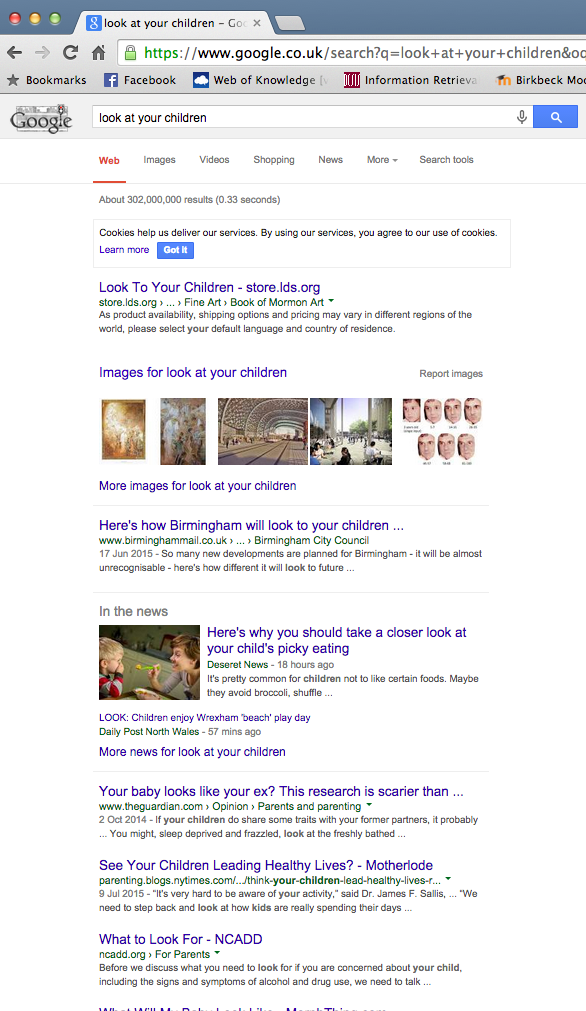
\includegraphics[width=.7\linewidth]{lookAtUrChildren}
  \caption{Incomplete query results.}
\end{subfigure}%
\begin{subfigure}{.5\textwidth}
  \centering
  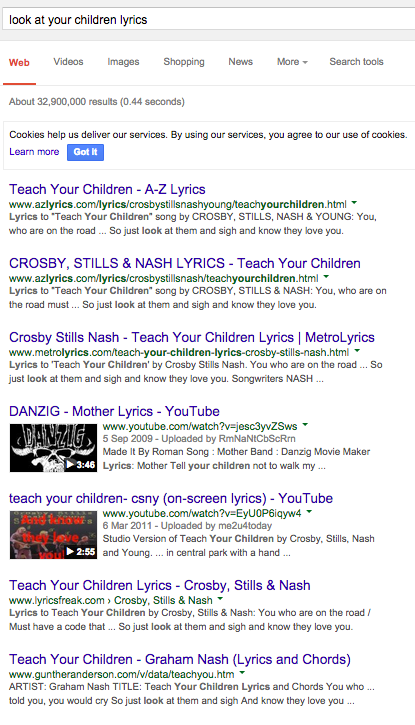
\includegraphics[width=.7\linewidth]{lookAtUrChildrenLyrics}
  \caption{Complete query results.}
\end{subfigure}
\caption{High and low AQ scorers both formed search queries accurately, however there was an increased tendency to omit the word ``lyrics" in the high AQ group resulting in very different search results.}
\label{someresults}
\end{figure}

\item{Although many high AQ scorers' formed query strings well, there was increased use of idiosyncratic words in the query strings that were formulated. This is in line with previous research that suggests that people with autism organise information in more subjective and individual ways \cite{subjective organisation}. For example, referring to the picture of the dog as `yorkie pooh'(not listed in frequency index), `aeroplane' (frequency of 8254 words per million) instead of plane (frequency of 33900 words per million) or flight (29535 words per million) , `miniature' (less than 4973 words per million) instead of small (185463 words per million). The idiosyncratic nature of the words is captured by their lower frequency of use in the English language. Search engines use term frequency to determine if a document is relevant to the users search query. If the frequency of words used to form search queries differs between low and high AQ scorers, so will the rankings of the returned search results.}
\label{idiosyncrasy}


\item{One individual of the 7 individuals in the high AQ group demonstrated ambiguous use of third-person pronouns, which is characteristic of some individuals with Autism \cite{pronoun}. This includes using first names. This is particularly detrimental to search engine query strings because the use of names disrupts the term frequency - inverse document frequency weighting \cite{tfidf} of the search query and subsequently the results returned to the user.
}\label{pronoun}
 
\item{
For questions that were `social' in nature (e.g., featuring a face of a famous woman), 2 out of 7 individuals in the high AQ group indicated that these were types of queries that they would not normally be interested in, and so ``wouldn't bother asking it". For these queries, it was more common for individuals in the high AQ group to include information in their search query string that was extraneous to the search question itself, compared to the low AQ group. For example, in query 4 above (which asked respondents to indicate how they would identify a famous person), 2 high AQ scorers included information about the woman's earring. Inevitably this `dilutes' the search query and results in reduced precision for the search engine.
}

\begin{comment}
\item{ 
Lastly there were more spelling errors and typographical errors in the high AQ group compared to the low AQ group.
}\label{spelling}
\end{comment}



\end{enumerate}


\subsection{Transforming the User Query.}
Given the set of observations in the data reported above, the aims were to `transform' queries made by individuals in the high AQ group to queries more similar to the low AQ group. The search engines already handle some of the observations from high AQ scorer queries. For example, the use of pronouns ('I' and `You') is already taken care of with the use of stop words. The aim of the project is to therefore address issues that result in the search query string being misleading, and returning differnt results to low AQ scorer search queries. The rule engine is a concrete and operationalised framework, for a theoretically-grounded stereotyped user model of autism within search. \\

\vspace{5mm} %5mm vertical space
Jellibeans works to address multiple observations made during the data collection stage, so the order in which the observations are tackled in the user model is not linear. As a general rule, changes will take the form of `add on' questions that aim to structure the individuals search query logically, so that key search terms are not dropped. A structured query formation will assist the user with less idiosyncratic search queries. \\


\vspace{5mm} %5mm vertical space

Building upon the reserach discussed in the introduction \cite{seo}, that search can be compartmentatlised into three broad categories (Do's, Know's and Go's), and, to address the observation of idiosyncrasy (point \ref{idiosyncrasy} above in the current research), Jellibeans will prompt the user to categorise their search query into one of 3 possible types of queries, a `Do', `Know' or, `Go'. `Do' queries are when they want to do something on the web like, buy a cinema ticket. `Know' queries for when they want to know something from the web like, what time the cinema closes. And, `Go' queries when they want to go somewhere specific on the web like the cinema homepage. Jellibeans will integrate a fourth subtype of query -- the `Social' query, especially for the user group in question. `Social' queries are for when their search is about something social; a person, or group of people. Social queries have additional functionality beyond the Do, Know and Go query pages, to reflect the additional difficulties individuals with Autism have when formulating Social search queries on the web.

\vspace{5mm}
Each type of query will be associated with a different colour, and once the user has selected that type of query, this colour will be prominent on the page throughout their search, to serve as a visual reminder of the task. This works to reduce the \textbf{working memory load} for the user, and to serve as a \textbf{goal-directed cue}. Two things we know are difficult for people with Autism are maintenance of information in working memory, and goal-directed tasks involving a high demand on Executive Functioning (Executive functions (also known as cognitive control and supervisory attentional system) is an umbrella term for the management (regulation, control) of cognitive processes, including working memory, reasoning, task flexibility, and problem solving as well as planning and execution \cite{EF}.) 

\vspace{5mm} %5mm vertical space

The Jellibeans `Social' query applies particularly to the user group in question, and has hints and suggestions added into search to assist the user when forming their query. The cues take the form of suggestions, that the user may select if helpful for their search, and to improve search results that are returned from Jellibeans.

\vspace{5mm} %5mm vertical space
To address observation \ref{incomplete}, that user queries were often submitted when incomplete, suggestions as well as drop down menus have been implemented on each search page. Users can click on suggestions, and select from the menus if they want the keyword to be added to their search. Individuals with Autism have an uneven cognitive profile, where verbal ability is usually lower than performance skill \cite{DSM}, the cues will assist users who have particular word-finding difficulties.


\vspace{5mm}
Once the user has pressed `Jellibean Search', and requested their search results be returned, Jellibeans collates all information the user has entered into the search boxes, as well as any suggestions, and options from drop down menu's that were selected to be included in the search. To achieve a good precision and specificity, Jellibeans implemented `AND' boolean operators between each input of the parametric search. This resulted in increased precision and a drop in recall for Jellibeans. The results are then presented to the user, with the exact phrase that was searched for. This means that the user can clearly see their final search query, and rather than a `black-box' system, Jellibeans also works to train the user for the long-term about specific ways to improve their personal search query strings. 

 \vspace{5mm}
 Because the current research identified that user's with Autism formed search queries were particularly incomplete for socially-grounded informational needs, extra functionality has been added to the `Social' query page. For example, if the user has indicated that they are searching for a famous person, they will be prompted for descriptions about that famous person's personality, character age bracket, and physical descriptions amongst other attributes. These features work to ensure that for this type of query, where users with Autism have most difficulty, that user search queries are more complete than they otherwise would have been (see Figure~\ref{socialCompleted}).

\begin{figure}[H]
\begin{center}
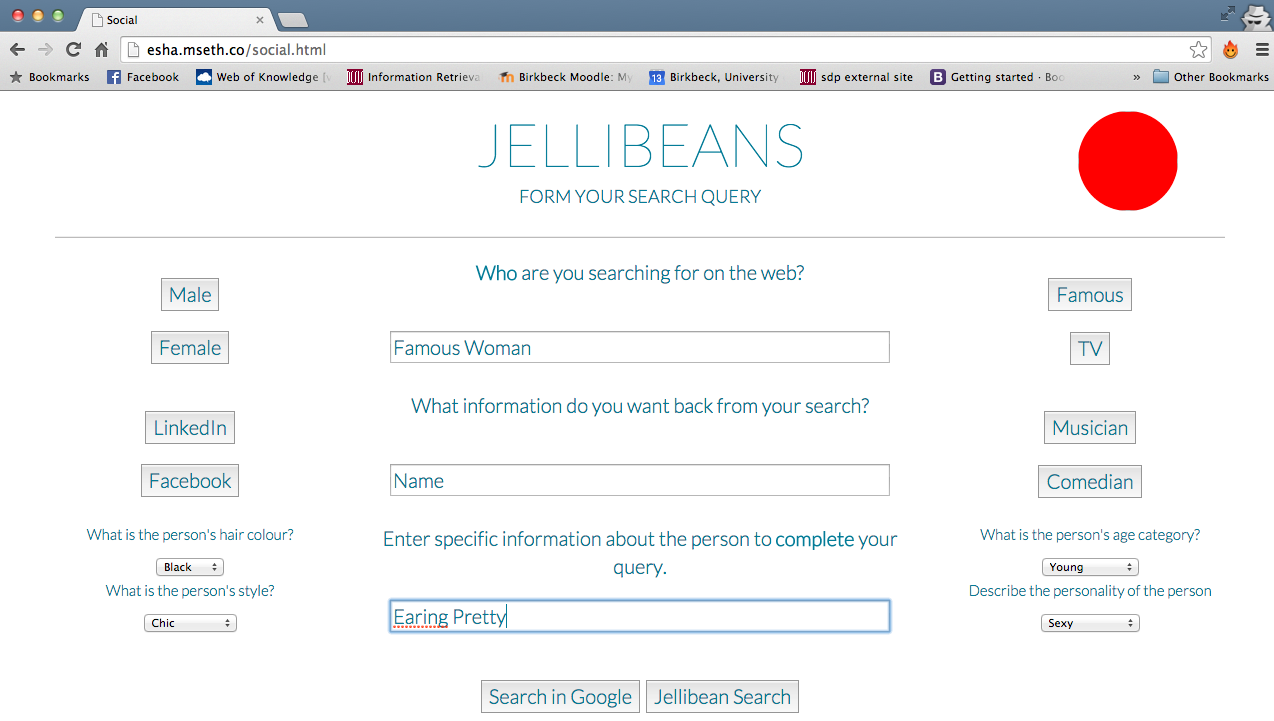
\includegraphics[scale=0.3]{SocialCompleted}
\caption{Example of User's Social Search in Jellibeans.}
\label{socialCompleted}
\end{center}
\end{figure}

\vspace{5mm} %5mm vertical space
To further address Core Feature 3 of Jellibeans, that is, that results should be returned to the user in smaller snippets rather than large sets of text, I modified the Jellibeans Custom Search Engine to select the 3 highest ranked (precision) results, and to present these back to the user on the first page of their search. The 3 top results are presented on a floating modal\footnote{A modal is a feature in the Bootstrap Framework, for more information see Appendix~\ref{implementation}}, so that the user has the option to close and reopen the results very easily, without having to redo the search itself (see Figure~\ref{resultsModal}).

\subsection{Storing the User Autism Score Data.}

The Autism Quotient score and all 50 of the responses from the user will be stored on a database (MySQL).


\begin{figure}[H]
\begin{center}
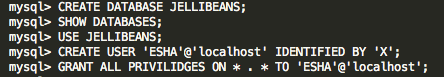
\includegraphics[scale=0.8]{mysql}
\caption{MySQL Used to Create and Query the Jellibeans Database.}
\label{mysql}
\end{center}
\end{figure}
[NEED TO INSERT MYSQL CODE HERE.]

\vspace{5mm} 
The user can also save their data locally to an Excel file by selecting the `Save Your Answers' button on the Jellibean Homepage (see Figure~\ref{saveScores}). Alternatively the user can choose `Calculate Your Score' which returns the score as an alert to the page.


\begin{figure}[H]
\begin{center}
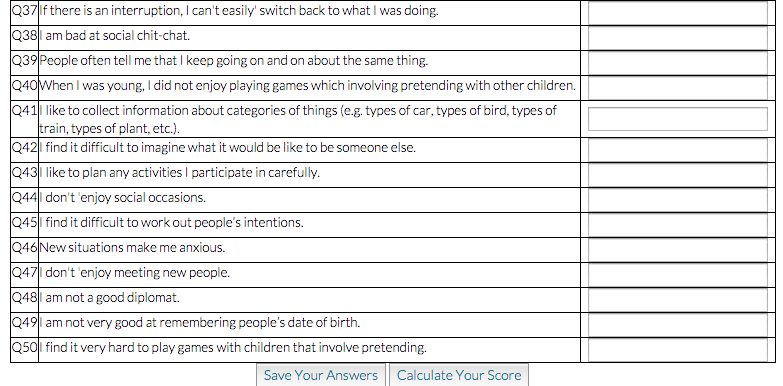
\includegraphics[scale=0.5]{saveScores}
\caption{The User Can Choose to Save Their Scores to an Excel File.}
\label{saveScores}
\end{center}
\end{figure}





\subsection{Integration with a Motion Controlled Interface.}

The selection process for the hardware to integrate with Jellibeans considered 4 factors; the timing of the device, the `volume', the applicability to real-world environments and the affordability for users.

\vspace{5mm}
Jellibeans is integrated with the LEAP Motion Controller Hardware (see Figure~\ref{leap}) which has good timing as it polls frames at a constant rate to keep to timining of accurate movement, and this is important for user experience. It is very easy to use and only requires a short calibration period. It is non-invasive and has a low sensory experience (sensory stimulation is not tolerated well by individuals with Autism). The cognitive demand needed to operate the LEAP is low, and given that web search is a highly cognitive task, this is of real benefit for the user.

\begin{figure}[H]
\begin{center}
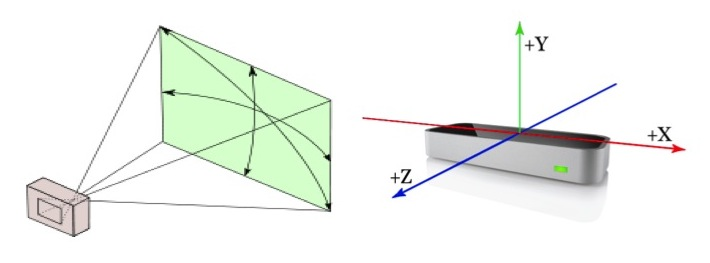
\includegraphics[scale=0.3]{leap}\\
\caption{The LEAP controller, with 150 degree view \cite{leap}.}
\label{leap}
\end{center}
\end{figure}

The LEAP recognises and tracks hands, fingers, finger-like tools, positions, motions and gestures using infrared light and optical sensors along the cartesian coordinate system. The controller has a 150-degree field of view, and operates in a range of 1 inch to 2 feet.  

\vspace{5mm}
Each of our senses operates with a different lag time. Hearing has the fastest sense-to-cognition/understanding, and surprisingly, sight -- the slowest. If the device interferes with the processing of the sense, it will confuse the combinatorial configuration of the senses, leading to misunderstandings in the meaning and a worse user experience. The LEAP does not have the best cognitive lag time compared to other devices such as the Oculus VR Rift. However, for Jellibeans, the browser refresh rate will likely be the biggest bottleneck for performance, rather than the motion-controller chosen. The LEAP is a completely non-invasive in comparison to the Rift (see Figure~\ref{vrVsLEAP}), so it was considered a better option for the current user group.

\begin{figure}[H]
\begin{center}
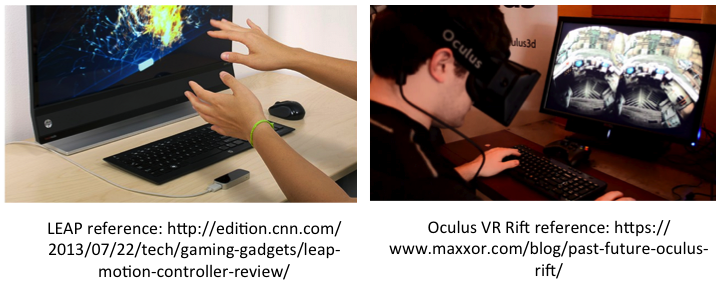
\includegraphics[scale=0.5]{VRvsLEAP}
\caption{Comparison of the invasivness of the Oculus VR Rift and LEAP motion controller.}
\label{saveScores}
\end{center}
\end{figure}

I also took into consideration the way in which the device manifests actions into behaviours. That is, how does the user engage behaviourally within the environment using the device? The LEAP was considered very realistic in terms of the transition of behaviour into real-world environments.

\subsubsection{Using LEAP in the IDE.}
Frames (cartesian coordinate data) from the LEAP were traked using the \texttt{Frames} class, and detected user motions. The following code was used to implement a forward-poking pointing motion to control mouse clicks. I ran the code to check how well it worked in Eclipse IDE (see https://youtu.be/ikfiul\_JPBk for a video of the LEAP working in my IDE). 

\begin{figure}[H]
\begin{center}
\includegraphics[scale=0.5]{leapCode}\\
\caption{Pointing and Poke Motion Used to Control Mouse Clicks.}
\label{leapCode}
\end{center}
\end{figure}

\begin{figure}[H]
\begin{center}
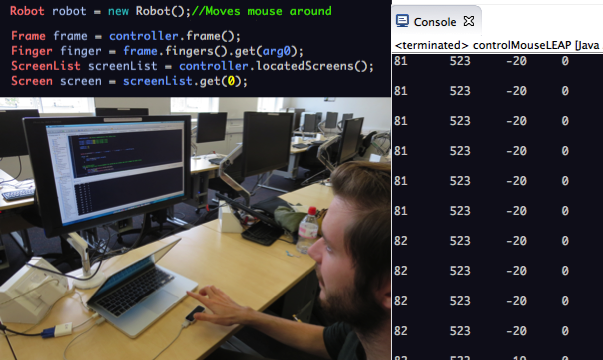
\includegraphics[scale=0.65]{Monty1}\\
\caption{Using the LEAP to Control the Cursor in the IDE. Console Output is Hand Coordinates along the x, y, and z Axes.}
\label{Monty}
\end{center}
\end{figure}

Although using the device this way was interesting and novel, the user has unstable control over the cursor, and often hand movements aren't precise enough to have a good experience using the hardware. I decided to look for a library that I could use with the LEAP to overcome this. One such library is LeapStrap which I discuss in the next section.


\subsubsection{Using LeapStrap in the Web-browser.}
To use the LEAP in a web-browser I used LeapStrap \cite{leapstrap}, which is built on top of Bootrap and was easy to integrate into the project. To integrate LeapStrap into the HTML I added link in the LeapStrap CSS , jQuery, Leap.js and LeapStrap.js. I also initialised the Leap in the body of the HTML code, and finally made all elements of the class ``leap-interactive" (see Figure~\ref{leapstrap}). 

\begin{figure}[H]
\begin{center}
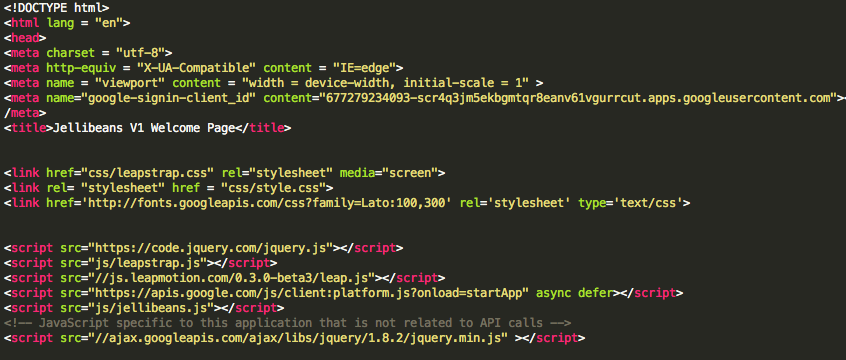
\includegraphics[scale=0.55]{leapstrap}
\caption{LeapStrap Library to Implement the LEAP for Jellibeans.}
\label{leapstrap}
\end{center}
\end{figure}

Once the LEAP was enabled for the web browser I was able to test Jellibeans with users to gather feedback. 

\begin{figure}[H]
\begin{center}
\includegraphics[scale=0.15]{OneHanded}
\caption{User Forming A Jellibean Search Query with LEAP Using One Hand.}
\label{OneHanded}
\end{center}
\end{figure}



\begin{figure}[H]
\begin{center}
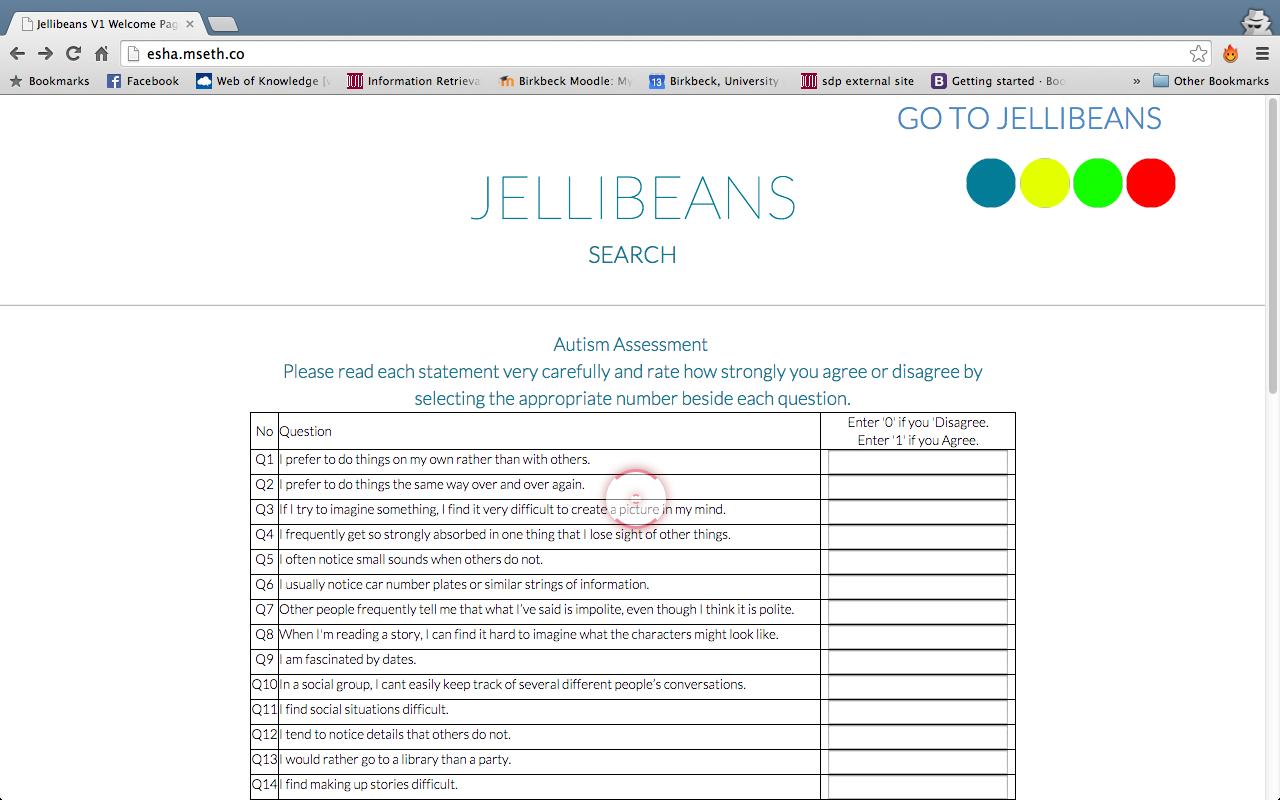
\includegraphics[scale=0.25]{leapweb}
\caption{Screenshot of how the LEAP projects a pointing finger onto the Jellibeans. Holding a finger pointer on a button for longer than a second, makes the pointer flash on the screen (indicating a mouse click has occured).}
\label{LeapOnTheWebsite}
\end{center}
\end{figure}

\section{Testing and Critical Evaluation of Jellibeans}
\subsection{Testing and Evaluation of the Combined Search Engine.}
To test the integrated combined search engine, 10 participants took part in a study to evaluate the quality of it's output. The participants were selected because they scored highly (above 30, where 32 is threshold for Autism Spectrum Disorder with a 79\% sensitivity) on a 50-item screening measure of Autism-like tratis (the Autism Quotient \cite{Baron Cohen et al}), and these individuals were thought to be most suited to test the current system. 

\vspace{5mm}
The range of scores for the AQ is 0 to 50 with high scores indicating increased likelihood of autism-like traits. A score under 21 is a low to average result (many women average around 15 and men around 17). A score of 22-25 indicates autistic tendencies slightly above the population average. A score above 26 gives a borderline indication of high functioning autism, or Aspergers. A score above 30 suggests a likelihood of Aspergers syndrome or autism (sensitivity of test measure = 79\% \cite{Baron Cohen et al}). For the purposes of this study, individuals with scores equal to, and above 30 were interpreted as having `autistic-like traits'.

\vspace{5mm}
Participants were asked to comment on their search results from 10 (pre-determined) informational needs. Participants were also asked to choose three out of the links returned that they would choose to follow up with. They were also asked if anything was odd about the results returned. The responses from the 10 users were then analysed. 

\vspace{5mm}
Somewhat non-surprisingly (given the statistics of most preferred search engines (Google's unique monthly visitors: 1,100,000,000 and query
volume: 64.5\% ; Bing: 350,000,000, 12.8\%; and Yahoo!: 300,000,000, 64.5\% (\cite{ebiz} \cite{adam})), the results revealed Bing Search was favoured the least, and Google results the most, with Yahoo falling somewhere in between. Out of the 30 responses participants indicated to follow up with (3 per participant), 21 were Google results, 3 were Yahoo, and 1 was Bing and 5 results overlapped between Google and Yahoo. Four participants commented specifically, that the Bing results were distracting rather than helpful.

\vspace{5mm}
Given these findings from the user group, future iterations of Jellibeans will continue using the Google results, but drop the results from Yahoo and Bing, in line with the aim of the project as a whole, that is, to improve returned search results for users with Autism.

\subsection {Evaluation of the LEAP Motion Controller in Jellibeans.}
The LEAP motion controller is an impressive device that uses infra-red light to embed the users (phantom) hands onto the screen. It is a novel, `at home' technology, and because of the portable nature of the device, it is one that has been introduced to laptops. The LEAP offers a recalibration process if the controller is persistently jumpy, which is good because jumpy movements and mannerisms could be an issue for some of the users in the current user group. The device will recalibrate if there are discontinuities or aberrations in the tracking data in certain field of view, or in poor tracking ranges. 

\vspace{5mm}
The LEAP does however miss small hand movements, and also very large ones (outside of the 150 degree angle along the y axis (see Figure~\ref{leap})). The LEAP also neglects to track the bottom left and right-most corners of the screen. I have tried to take this into consideration when designing Jellibeans, so that the user does not need to reach to the corners of the screen.

\section{Software Testing}


I used Behaviour Driven Development (BDD) to test the integration of my HTML, CSS and JavaScript code. The testing process consisted of development, test, make modifications, test (and so on) until the behaviour of the website was what I intended.\\

\vspace{5mm}
The JavaScript Console was used for testing JavaScript code. \cite{javascripttesting}, I also used JSfiddle \cite{jsfiddle} to ensure the code contained no bugs, and was particularly good for seeing how the JavaScript code integrated with the HTML code and CSS.

\vspace{5mm}
JUnit was used to test the Combination Search Engine and the LEAP motion controller methods, which were written using Java. Test Driven Development unit testing was completed, at the level of each method implemented.


\begin{comment}
\vspace{5mm}
TODO consider using CUCUMBER IN ECLIPSE.https://hjrlive.wordpress.com/2014/02/15/test-post/
\end{comment}

\section{User Verification and User Testing}
Five high AQ scorers were called back from the previous research study for one-to-one interviews and a combined focus group. During the interview, individuals were given the same user search queries as previously, and for each search that was implemented, users were asked to comment on whether it enhanced, or took away from their search experience, and from their satisfaction with the search results. 

\subsection{Interviews}
\subsection{Quantifiable results}
The 5 participants were asked to re-construct the same search queries they had been asked to construct in the first research study, using the search engine they identified as their usual choice (all participants said they would usually Google), and also using Jellibeans. 

\vspace{5mm}
Participants were asked to comment on:
\begin{itemize}
\item{Whether they found a result they would be satisfied with using both search tools, Jellibeans only, Google only, or neither.}
\item{Which search tool gave them the most relevant results overall, and how many were relevant (focusing only on the top 3 links for comparison purposes, as Jellibeans only returns 3 results.)}
\end{itemize}

\vspace{5mm}
The search strings that these users formulated are presented below.


\textbf{Search strings formed by users with Autism, \underline{without using Jellibeans}. }
\begin{enumerate}\label{asdresponses}
\item{You hear a song on the radio with the lyrics, `Look at your children', and you want to download it. What would you type into search on your favourite search engine to find out what song it was?\\\textit{Song lyrics look at your children\\
look at your children\\
Look at your children song\\
``Look at your children" lyric\\
Look at your children\\
``Look at your children" lyrics\\
Look at your children song\\}}
\item{You've lost touch with an old school friend (you went to St. Mary's School). What key words/queries would you use to find them?\\\textit{*Persons name* and St Mary's school on Facebook\\Full name of friend, St Mary's School, year of graduation (i.e. `class of')\\
The friend's full name and ``St. Marys"\\
Me and St Marys\\
I wouldn't want to know. I wouldn't bother\\
St Mary's school with the year we left \\
Google their name}}
\item{How would you identify what this is using a search engine (pretend you don't know what it is called). What key words/queries would you use?\\\textit{Google image search, or failing that: dried herb star 8 points\\
Star shaped seed pod\\
Star eight spice wikipedia\\
Star shaped flower \\
Wooden flower\\
Star shape hard shell \\
Post a picture on Facebook\\
No answer}}
\item{How would you find out the name of this famous person using a search engine? What key words/queries would you use?\\\textit{Pale brunette brown(or hazelnut) eyes freckles natural beauty earring\\
Not something I would search for\\
Model actress long brown hair, brown eyes, big lips\\
Celebrity female young long dark hair earring\\
I wouldn't expect to be able to find out their name unless I had more information than just a physical description\\
Famous females\\
Pretty white brunette \\}}
\item{How would you identify what breed this animal is using a search engine? What key words/queries would you use?\\\textit{Small dog breeds terriers\\
Small dog fluffy head moustache breed\\
Dog breed grey furry miniature\\
Yorkie pooh \\
Small pet dog\\
Small dog fluffy head moustache breed\\
`Small dog breeds' }}
\item{Your friend and you can't agree on how Thandie Newton pronounces her first name. How would you resolve this using a search engine?\\\textit{Interview with Thandie Newton\\
Pronounce `Thandie Newton'\\
How to pronounce Thandie Newton\\
Thandie Newton pronunciation\\
`Thandie Newton pronunciation'\\
Thandie Newton\\
YouTube Thandie Newton}}
\item{What would you search for to identify this pattern's name, and which country it originates from?\\\textit{Some combination of: tiling symmetry \\
Tessellating ``interlocking s"\\
Square spiral repeating pattern name origin\\
Square spiral originates from\\
Repeating square patten\\
5 part wave pattern square \\
Celtic patterns}}
\item{How would you search for delay's relating to your (imminent) flight to Paris?\\No answer given\\\textit{
Airport website\\
Flight number plus the date and time\\
Aeroplane\\
Departures from airport X\\
Search for confirmation email in my inbox\\
Paris departure Heathrow\\
}}
\end{enumerate}


\textbf{Search strings formed by users with Autism, \underline{with Jellibeans}. }
\begin{enumerate}\label{asdresponses}
\item{You hear a song on the radio with the lyrics, `Look at your children', and you want to download it. What would you type into search on your favourite search engine to find out what song it was?\\\textit{
Name of song song name Look at your children Music\\    
Song lyrics look at children Listen \\
Lyrics for song  look at your children \\      
Song name look at your children song \\      
Name of song name of song look at children 	
}}
\item{You've lost touch with an old school friend (you went to St. Mary's School). What key words/queries would you use to find them?\\\textit{
School friend name st marys school Female Brown hair Middle aged \\ 
Name of friend from st marys name class of x Female \\        
Friend name st marys school Female Middle aged  \\
Name st mary school Male Facebook black hair Middle aged Modest \\
Name of friend from st marys name 
}}
\item{How would you identify what this is using a search engine (pretend you don't know what it is called). What key words/queries would you use?\\\textit{
Name of star shape brown shell edible item \\        
Wikipedia name of star eight spice \\    
Dried herb star eight spokes and spice \\        
Organic brown star name flower \\       
Name of  organic spice wikipedia  natural wooden     
}}
\item{How would you find out the name of this famous person using a search engine? What key words/queries would you use?\\\textit{
Famous lady with brown hair name Brown Young Chic Sexy\\
Brown eyes woman Famous Female Brown Young Modest Moody\\
Actress pale brunette natural Female Brown Middle aged \\
Celebrity female long hair dark earring name Famous Female Brown Middle aged Serious \\
Pretty white brunette name Famous Female Brown Young Chic
}}
\item{How would you identify what breed this animal is using a search engine? What key words/queries would you use?\\\textit{
Name of small white fluffy dog name \\       
White dog small poofy hair name \\      
Name of dog white small  yorkie  \\
Grey and white dog small  name of dog \\
Pet dog name name white small moustache breed      
}}
\item{Your friend and you can't agree on how Thandie Newton pronounces her first name. How would you resolve this using a search engine?\\\textit{
Thandie Newton interview YouTube \\    
How to pronounce Thandie Newton name pronunciation \\
Pronounce Thandie Newton name \\
Thandie Newton's name how to say it\\
Thandie Newton pronunciation YouTube   
}}
\item{What would you search for to identify this pattern's name, and which country it originates from?\\\textit{
Name of pattern country of origin name blue spiral \\     
Origin of pattern country name repeating pattern  spiral Wikipedia \\     
Name repeating pattern  symmetry tile   Wikipedia \\
Tessellating interlocking s pattern origin Wikipedia \\ 
Repeating pattern tile symmetry Wikipedia name of pattern   
}}
\item{How would you search for delay's relating to your (imminent) flight to Paris?\\No answer given\\\textit{
Flight number information Ryan air to Paris  Homepage \\
Departures from London to Paris airlines information delays \\
Aeroplane flight delays paris departure Heathrow \\     
Departure to paris flight delay  information \\
Airport website flight delay to Paris  
}}
\end{enumerate}

\subsubsection{Result 1}
The first question was whether participants found results they would be satisfied with using both search tools, Jellibeans only, Google only, or neither.

\vspace{5mm}
\begin{itemize}
\item{For each question the defining criteria of a succesful search was defined according to the base model (from typically developing individuals):}
\subitem{A reference to the `name of the song' / `lyrics' and `Look at your your children'.}
\subitem{A reference to `St Marys School', [year of graduation] and a description of the person.}
\subitem{Reference to the `star' shape, the colour `brown', and the fact it was a `plant'/`organic'.}
\subitem{Reference to a famous woman with brown hair and young. }
\subitem{Reference to a `small' `dog', and `fluffy' breed.}
\subitem{A query with the keywords `Thandie Newton' and `Pronunciation'}
\subitem{A reference to a `square pattern' which is `repeating' (`tiles' or `spiral' interchangably used), with `origin'. }
\subitem{A reference to `Paris', `airport/aeroplane', `flight time/information'.}
\end{itemize}

A categorical analysis was conducted to validate the search efficacy of Jellibeans. There 40 queries in total. Participants were asked to consider the top 3 results from Google (for comparison with Jellibeans), and to explain if their search was satisfied by Jellibeans (only), their other search tool of choice (only), both, or neither. The graph below demonstrates that Jellibeans has a good precision rate (30\%) compared to other search tools (25\%), see asterix Figure ~\ref{result1}, although this was not a significant difference (see Figure ~\ref{result1spss}).
\begin{figure}[H]
\begin{center}
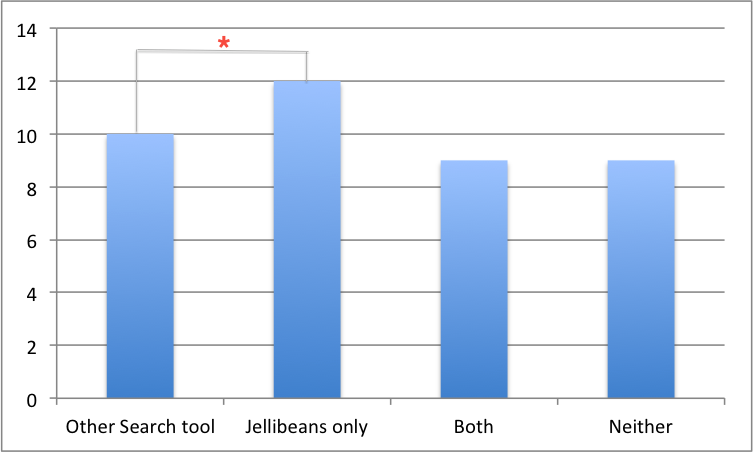
\includegraphics[scale=1]{Result1star}
\caption{Y axis represents the number of search queries correctly retrieved (out of a possible total of 40). X axis shows number for each search tool, both or neither.}
\label{result1}
\end{center}
\end{figure}

\begin{figure}[H]
\begin{center}
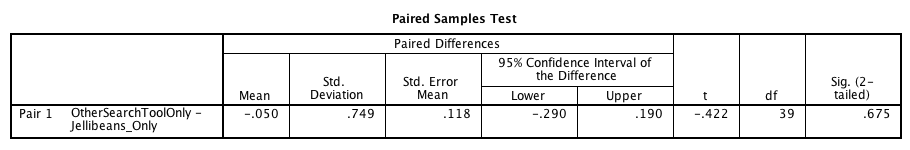
\includegraphics[scale=0.47]{Result1spss}
\caption{No significant difference in precision of Jellibeans compared to other search tools, when considering only the top three results.}
\label{result1spss}
\end{center}
\end{figure}

The full data file can be found in Appendix~\ref{datacoding}.

\vspace{5mm}
This means that Jellibeans is successfully reducing the number of results the participant has to sift through - down to just 3 results - without reducing precision of the search tool within those items.

\subsubsection{Result 2}
Participants were asked to count the number of results (in the top three) that they felt were relevant to the search query. These data are presented in Figure ~\ref{result2}. The results show that the recall was comparable (albeit variable) between Jellibeans and the usual search tool for the participant.

\begin{figure}[H]
\begin{center}
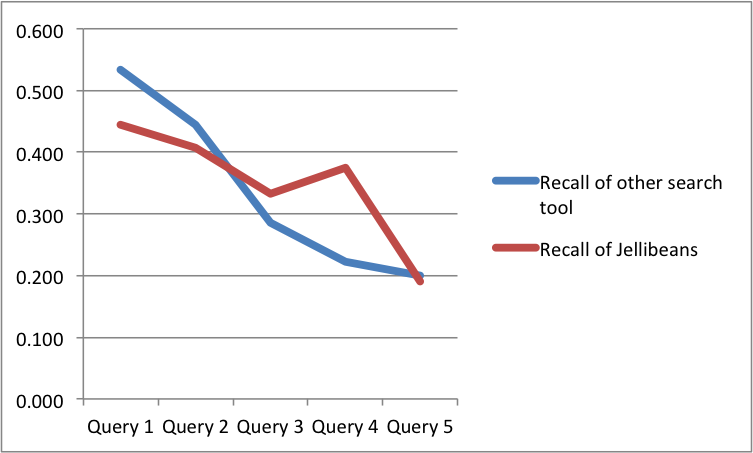
\includegraphics[scale=1]{result2}
\caption{Recall for Jellibeans versus the usual participant search tool.}
\label{result2}
\end{center}
\end{figure}

\subsubsection{Result 3}
There was a significant difference in the number of words used to form search queries when comparing Jellibeans to other search tools. Significantly more words were used to form search queries using Jellibeans (mean number of words in Jellibeans = 3.53, mean number of words in other search tools = 6.55). A paired-samples t-test was run to confirm this observation (t = -7.79, df = 39, p $<$ 0.001, see Figure~\ref{result3}). This is interesting because it means that individuals use more words and to narrow down the scope of their search, which is useful for increasing precision scores of the search tool.

\begin{figure}[H]
\begin{center}
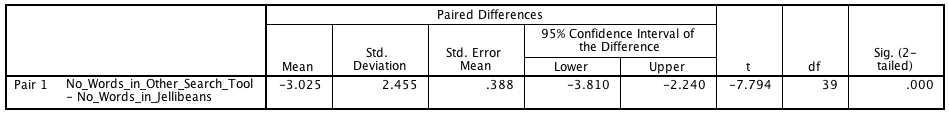
\includegraphics[scale=0.47]{Result3}
\caption{Result of t-test comparing number of words used to form search queries. Participants used more words to define their queries using Jellibeans compared to other search tools.}
\label{result3}
\end{center}
\end{figure}

There was also more repetition in words used to form search queries in Jellibeans. This is probably due to the nature of the search process using this tool -- there are more search inputs to complete and drop down input boxes (to select `keywords') which are added to the search in Jellibeans. To remove this confound, keywords that were repeated were dropped from the analysis.

\vspace{5mm}
This means that individuals are defining their search queries using more keywords in Jellibeans. This is most likely the reason why Jellibeans is able to maintain a good precision, with only three keywords returned to the user. 


\subsection{Focus Group}
During the focus group users were asked to comment on:
\begin{enumerate}
\item{Whether the colour coding for each category of search was helpful.}
\item{Whether they liked the parametric search style of Jellibeans}
\item{Whether they felt Jellibeans `narrowed' the scope for irrelevant detail.}
\item{If they would choose Jellibeans over other search engines, for example, Google, and why.}
\item{The speed and efficiency of search with Jellibeans}
\item{Their thought on search results.}
\item{The integration of Jellibeans with the LEAP motion controller.}
\end{enumerate}

\subsubsection{The Positives}
All 5 users verified that the `Dashboard' colour coding was helpful (see Figure~\ref{colourCoding}), and liked that the colour of the chosen type of search remained on screen for its duration.

\begin{figure}[H]
\begin{center}
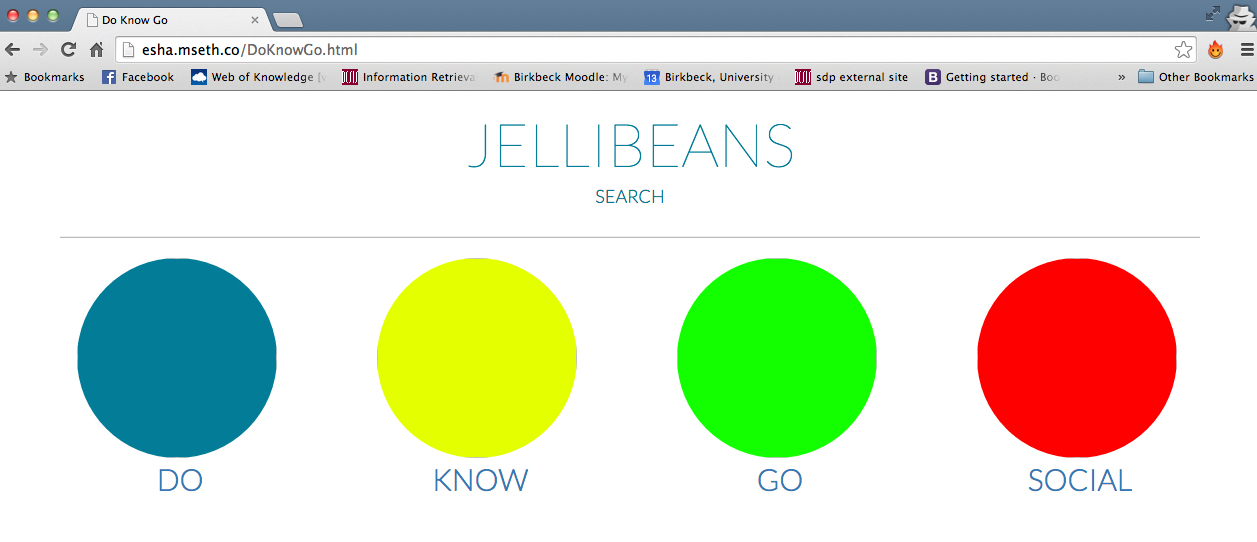
\includegraphics[scale=0.25]{DoKnowGoSocialDashboard}
\caption{Colour coding on Jellibean dashboard.}
\label{colourCoding}
\end{center}
\end{figure}

The modals (floating window reminders) for each of the colour themes were useful for all new users, as they were originally unfamiliar with the colours. The associations for all user groups, including users with Autism, were quick to learn, these were single link visual (rather than verbal) associations.\\

\begin{figure}[H]
\begin{center}
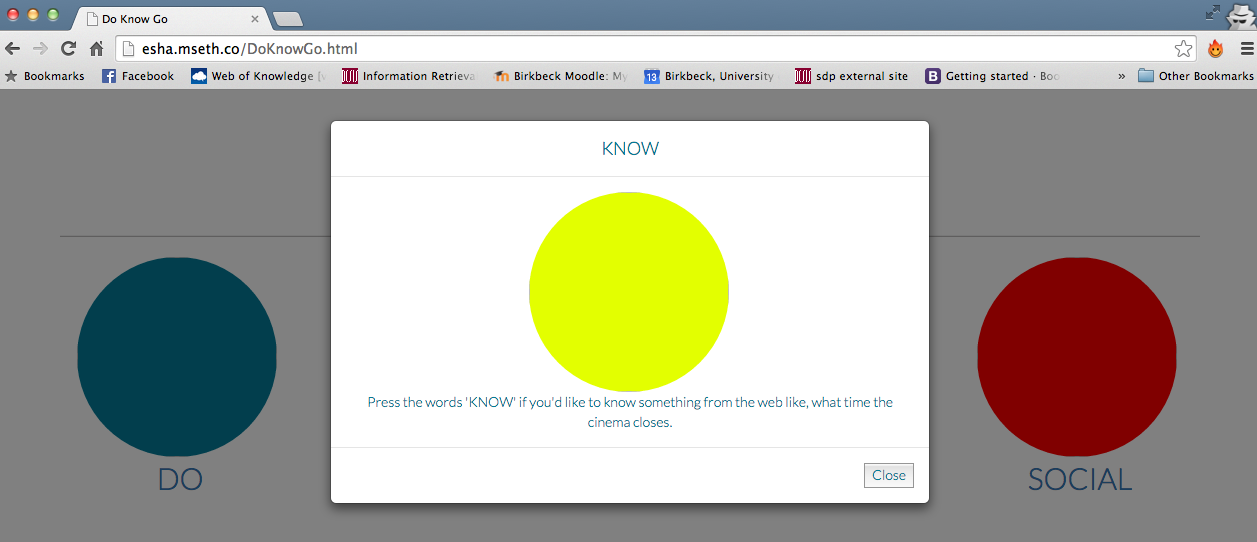
\includegraphics[scale=0.25]{floatingModals}
\caption{Modals Assist New Users To Lean the Colour Associations.}
\label{colourCoding}
\end{center}
\end{figure}


Four out of 5 participants agreed that one of the major positives of Jellibeans was that unlike Google, users did not receive back hundreds and thousands of mostly irrelevant results. Jellibeans held their interest for longer because of the reduced number of results that users had to sift through. Testing also revealed that the parametric search style meant that they did not need to try and remember all the key words to search for, rather the cues helped them remember points they would have missed otherwise. \\

\vspace{5mm}
A common comment (3 out of 5 users) was the time/reward payoff from completing a detailed search form. Users agreed that although they would spend more time formulating their search query, they were likely to save time that would usually be spent sifting through search results. These participants indicated that they would use Jellibeans over other search engines if continued use on other queries also showed such benefit.\\

\vspace{5mm}
All users positively commented on the reduced number of search results presented (top 3). The amount of textual information that was presented back on the results page is significantly reduced in Jellibeans. 

\vspace{5mm}
During the focus group one user with high functioning Autism described that the direct questions (e.g., `What do you want to do on the web?'), with suggestions (`Shop', `Watch', `Listen'), was useful when he was ``at a total blank". He disclosed that often his need for perfectionism and sameness could have him staring at a blank screen until he came up with the `perfect' query. However, the suggestions were helpful for him to get started, and so his experience was that the queries were completed faster than usual.  \\

\subsubsection{The Negatives}

Two users however, had considerations about the `missing' results from their search and commented that for them, 3 results were too few and perhaps 5 or 6 results would have been a better choice. It must be said that these individuals were amongst the lowest AQ scorers, suggesting that the amount of text individuals with Autism find optimal is a function of the severity of Autism traits in that individual.

\vspace{5mm}
One participant commented that the suggestions that appear on the sides of the `Do', `Know', `Go' and `Social' pages were not user-specific (see Figure~\ref{suggestions}). He suggested implementing something that is user-centred, user-driven, or, trending, rather than static.

\begin{figure}[H]
\begin{center}
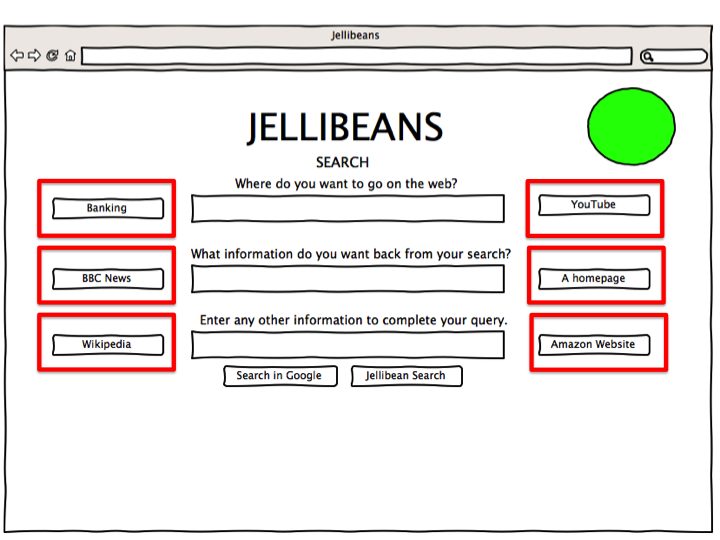
\includegraphics[scale=0.3]{suggestions}\\
\caption{Suggestions on Jellibeans `Go' page for users to help with search query formulation (suggestions are highlighted in red).}
\label{suggestions}
\end{center}
\end{figure}

However, one of the characteristics of Autism is restricted and repetitive behaviours, and an aims of the current project was to reduce the restricted and repetitive nature of search queries for people with Autism. In other words, this comment was suggesting that Jellibeans was achieving the aim it had set out to do.

\vspace{5mm}
Nevertheless, one future direction for Jellibeans in order to achieve a balance between user-specific suggestions but not restricted interests, is to include a recommendation system that changes often enough for them not to be repetitive, but still within a range of possible interests for that individual. 

\subsubsection{Other observations}

Users agreed during the focus group that with Jellibeans the time/reward payoff is really only apparent, over and beyond a traditional search engine, when the search query is complex. For example, if users are searching for something they have yet to identify, i.e., something ambiguous. To overcome this criticism, Jellibeans includes a `Search in Google' option, so that if users know what they are searching for, they have the option to run the search outside Jellibeans.

\begin{comment}
\vspace{5mm}
Describe the verification process you used in your project\\
Unit Testing, Static Analysis for methods in javascript etc.\\
Manual testing, Selenium, Cucumber etc for html.\\
Regression tests
\end{comment}


\section{Evaluation and Discussion.}\label{eval}

Several unexpected challenges and successes occured during the course of the project's execution.  

\subsection {Challenges}
One challenge was encountered when integrating the Apache Lucene Library with Jellibeans. The library was not well maintained and the org.apache.log4j file log was broken. I considered Apache Solr \cite{solr}, and Apache Nutch \cite{nutch}, but these libraries requires a large document collections to create indices prior to text search. It was not feasible to index the entire document colletion on the web for Jellibeans, and to sift the web \textit{on the fly} would have resulted in a long duration for participant user queries. To overcome this challenge I followed the mitigation protocol outlined in my project proposal that stated I should attempt to implement the methods needed. User testing showed that the implemented solution was senstive enough to retrieve documents that satisfied user search queries.

\vspace{5mm}
It was originally thought that user Autism Scores would be stored in their Google+ profile, to be retrieved when users sign in to Jellibeans using Google+. However, Google+ did not allow for a field to persist after the session ended to retrieve the user's score. Conversely, any data stored to Google+ would not be retrievable after the user's session had ended (i.e., after the user logged out of Google+). To overcome this challenge I implemented my own datastore for user's Autism Quotient Scores. The final prototype of the application is therefore integrated with Google+ and this additional datastore (although in prototype models only Google+ was integrated with Jellibeans).

\vspace{5mm}
To deploy the application, with a database in the web browser, I learned a number of development languages that I had not used before. This included php, JQuery, JavaScript, HTML and CSS. I worked with a new php frameowrk called Laravel\cite{laravel} to deploy the application in the browser. Although the prototype of Jellibeans (at esha.mseth.co) is implemented using static HTML, I chose to implement the final application using this dynamic website framework. This was one of the biggest personal challenges of the project, and steepest learning curve. 

\vspace{5mm}
Web Robots automatically traverse the web to retrieve a document, and in a recursive fashion these robots retrieve all documents that are referenced. This does not include web searches, which are operated by human queries, as these are not programatically requested but instead are genuine user and human queries. \\
However, when Jellibeans was implemented programatically from Eclipse IDE \cite{eclipse}, I often received blocked requests in the console. This was because several websites implement \texttt{robot.txt} files to block web crawlers. This was a challenge that was unexpected and originally seemed unsurmountable. After some research it became apparent that to overcome this challenge, I needed to register Jellibeans as a project in the Google Developers Console \cite{GDC}, after which correct privilidges would be assigned.

\begin{comment}
Sandboxes
\end{comment}

\subsection{Successes}
During the course of the project, user testing was conducted on 52 occasions (surveys = 37 participants, feedback on combined search engine = 10 participants and interviews/focus group = 5 participants). Seven of the individuals who participated in the survey had an increased Autism Score, and 5 of these individuals were included in the feedback stages of user testing for Jellibeans. 

\vspace{5mm}
User testing demonstrated that the user model that Jellibeans implements works well in the search tool. Participants reported a number of positives with the application that shows promise for the future development of Jellibeans.

\vspace{5mm}
The LEAP integrated behaviour into the web browser in a very naturalistic way. The movements are smooth and the visual aesthetics of the pointer on the screen are a gret balance of fun, \textit{and} function. The cursor is easy to use even for people with uncontrolled, or, jerky hand movements. 

\vspace{5mm}
Although not part of the original proposal for the project, and even with a number of challenges along the way, there was time to implement some of the user feedback to drop frustations that users identified during user testing before the final prototype was implemented. Other modifications suggested by users required the purchase of data (such as `current trends') which I have spoken about in Section {future}.

\subsection{Future Directions}\label{future}
There are many avenues to consider for the future of Jellibeans. For example, modifications to the asthetic appeal, user needs, and functionality of the application.

\vspace{5mm}
A future aesthetic consideration is to improve the visual design of the website itself. In the current version Bootstrap was used, which helped considerably with visual aesthetics, however this could be further considered along with functionality as well. If I were to redesign Jellibeans, I would not present the Autism Questionnaire on the first page of the application, but instead have this on a separate page. I would also choose to implement an abbreviated version of the test, or a version for parents or carers to complete on behalf of the user (as a 50-item optional questionnaire may not have the best response rate from individuals with Autism themselves).

\vspace{5mm}
A future functional direction for Jellibeans would be to use an API or library for word frequencies in the written English language, which could be integrated with a thesaurus. This type of API requires significant research into the natural language processing of written (rather than spoken) English text. These frequency data could have been used to replace infrequent words in queries formed by individuals with Autism with more frequent words to suggest alternatives for the user. Of course this product would not be scalable, and only apply to users with a particular dialect. This is because word frequency is considerably variable across, and even within a language (e.g., consider South-West England compared to the North of England).

\vspace{5mm}
Another future direction for Jellibeans would be to implement current trending searches, which could be a contributing factor in the future for why users choose other search engines over Jellibeans. 

\vspace{5mm}
Individuals with Autism have increased comorbidity with Attention Hyperactivity Disorder (ADHD), and Colour Blindness, and so these can be taken into account for future iterations of Jellibeans. For example, the colours used for Jellibeans are in the RGB colour scheme, but these could be replaced with gradients or patterns so that individuals with colour blindness can also also benefit.





\clearpage
\begin{thebibliography}{100}

\bibitem{Baron Cohen et al} Baron-Cohen, Wheelrigjt, Skinner, Martin, Clubley (2001).  The Autism-Spectrum Quotient (AQ): evidence from Aspergers Syndrome/high-functioning autism, males and females, scientists and mathematicians.  \textit{Journal of Autism and Developmental Disorders, 31}, 5-17.
\bibitem{bootstrap}Bootstrap, http://getbootstrap.com/ Retrieved September 2 2015
\bibitem{attention} Bronwyn, M, Murray, M, and Durkin, K. (2003) Weak central coherence, poor joint attention, and low verbal ability: Independent deficits in early autism. \textit{Developmental Psychology, 39}, (4), 646-656. http://dx.doi.org/10.1037/0012-1649.39.4.646
\bibitem{subjective organisation} Bowler, D. M., Gaigg, S. B., Gardiner, J. M. (2008). Subjective organisation in the free recall learning of adults with Aspergers syndrome. \textit{Journal of Autism and Developmental Disorders, 38}(1), pp. 104-113. doi: 10.1007/s10803-007-0366-4 
\bibitem {CDC}Developmental Disabilities Monitoring Network Surveillance (2010) \textit{Centers for Disease Control and Prevention (CDC). Prevalence of autism spectrum disorders: Autism and Developmental Disabilities Monitoring Network, United States. MMWR Surveill Summ.2009; 58},
\bibitem {DSM}Developmental Disabilities Monitoring Network Surveillance (2010) \textit{Centers for Disease Control and Prevention (CDC). Prevalence of autism spectrum disorders: Autism and Developmental Disabilities Monitoring Network, United States. MMWR Surveill Summ.2009; 58}, 10:120
\bibitem{eclipse} Eclipse Luna IDE, https://eclipse.org/luna/, Retrieved 27 August 2015.
\bibitem{ebiz}eBizMBA inc, \textit{The eBusiness Guide}, www.eBizMBA.com; Retrieved 20 March 2015
\bibitem{EF} Executive Function, https://en.wikipedia.org/wiki/Executivefunctions, Retrieved 27 August 2015.
\bibitem{disengagement}
Elsabbagh, M., Volein, A., Holmboe, K., Tucker, L., Csibra, G., Baron-Cohen, S., Bolton, P., Charman, T., Baird, G. and Johnson, M. H. (2009), Visual orienting in the early broader autism phenotype: disengagement and facilitation. \textit{Journal of Child Psychology and Psychiatry, 50}, 637–642. doi: 10.1111/j.1469-7610.2008.02051.x
\bibitem{seo} Fishkin (2015) https://moz.com/beginners-guide-to-seo/how-people-interact-with-search-engines, Retrieved 3 August 2015.
\bibitem {gameshealth} Games for Health (2012) \textit{Screen-based technologies and Autism. 1}: 248-53
\bibitem{leap} Leap Motion, \textit{Java SDK Documentation}, \\https://developer.leapmotion.com/documentation/java/index.html Retrieved 1 April 2015.
\bibitem{GDC} Google Developers Console, https://console.developers.google.com, Retrieved 1 April 2015.
\bibitem{leapstrap} LeapStrap, http://wilkesalex.github.io/leapstrap/getting-started/, Retrieved September 3 2015.
\bibitem{motioncontrollerforautism} Garzotto, F., Valoriani, M. and Bartoli, L. (2014), Touchless Motion-Based Interaction for Therapy of Autistic Children, Virtual, Augmented Reality and Serious Games for Healthcare, \textit{Intelligent Systems Reference Library, 68}, 2014, pp 471-494
\bibitem{googleTerms} Google Privacy and Terms, http://www.google.com/policies/technologies/, Retrieved 27 August 2015.
\bibitem{javascripttesting} JavaScript Console, https://developer.chrome.com/devtools/docs/console, Retrieved September 3 2015.
\bibitem{jsfiddle} JS Fiddle, https://jsfiddle.net/, Retrieved September 3 2015.
\bibitem{jsoup} JSoup Java API, http://jsoup.org/, Retrieved 27 August 2015.
\bibitem{laravel}Laravel, laravel, http://laravelbook.com/laravel-architecture/ Retrieved Sep 6 2015
\bibitem{mottron}Laurent Mottron, Jacob A. Burack, Johannes E. A. Stauder, Philippe Robaey (1999) Perceptual Processing among High-functioning Persons with Autism. \textit{Journal of Child Psychology and Psychiatry 40}, (2), 203211. doi:10.1111/1469-7610.00433.
\bibitem {adam}Lella, A., (2014). \textit{comScore Releases March 2014 U.S. search Engine Rankings.} ComScore.com. Retrieved 21 Feb 2015
\bibitem{moore}Moore, D. J., McGrath, P., \& Thorpe, J. (2000). Computer aided learning for people with autism—a framework for research and development. \textit{Innovations in Education and Training International, 37}
\bibitem{pronoun} Novogrodsky, R. (2013). Subject-pronoun use of Children with Autism Spectrum Disorders (ASD). \textit{Clinical Linguistics and Phonetics, 27}(2), 85-93. 
\bibitem{nutch} Apache Nutch, http://nutch.apache.org/, Retrieved September 10 2015.
\bibitem {opensearch}OpenSearch, http://www.opensearch.org/Specifications/OpenSearch/1.1, Retrieved 30 July 2015.
\bibitem{phptester} Online PHP tester, http://phptester.net/, Retrieved September 7 2015.
\bibitem {Shane and Albert}Shane, H. C. and Albert, P. D. (2008) Electronic screen media for persons with autism spectrum disorders: results of a survey. \textit{Journal of Autism Developmental Disorders, 38},8 :1499-508. doi: 10.1007/s10803-007-0527-5.
\bibitem{AdultsWithAutism} Slavin, S (2013) Autism: Successful communication,10 things to make it easier, http://adultswithautism.org.uk/autism-successful-communication-10-things-to-make-it-easier/, Retrieved September 1 2015.
\bibitem{solr} Apache Solr, http://lucene.apache.org/solr/, Retrieved September 10 2015.
\bibitem{surveymonkey}Surveymonkey, https://www.surveymonkey.com/home/, Retrieved 5 August 2015.
\bibitem{tfidf} Term Frequency Inverse Document Frequency Weighting, http://nlp.stanford.edu/IR-book/html/htmledition/tf-idf-weighting-1.html, Retrieved 9 August 2015.
\bibitem{wordfrequncy} Word Frequency Information, http://www.wordfrequency.info/free.asp?s=y, Retrieved 6 August 2015.
\bibitem {usermodel}Shen, X., Tan, B. and Zhai, C. (2005) Implicit User Modeling for Personalized search, \textit{Conference on Information and Knowledge Management}, Bremen, Germany.
\end{thebibliography}





\newpage
\section {Appendices}

\begin{comment}
\newpage
\subection{}\label{}
\begin{figure}[H]
\begin{center}
\includegraphics[scale=0.55]{}
\caption{}
\end{center}
\end{figure}
\end{comment}

\newpage
\subsection{Class Diagram}\label{jBeanClassDiagram}
\begin{figure}[H]
\begin{center}
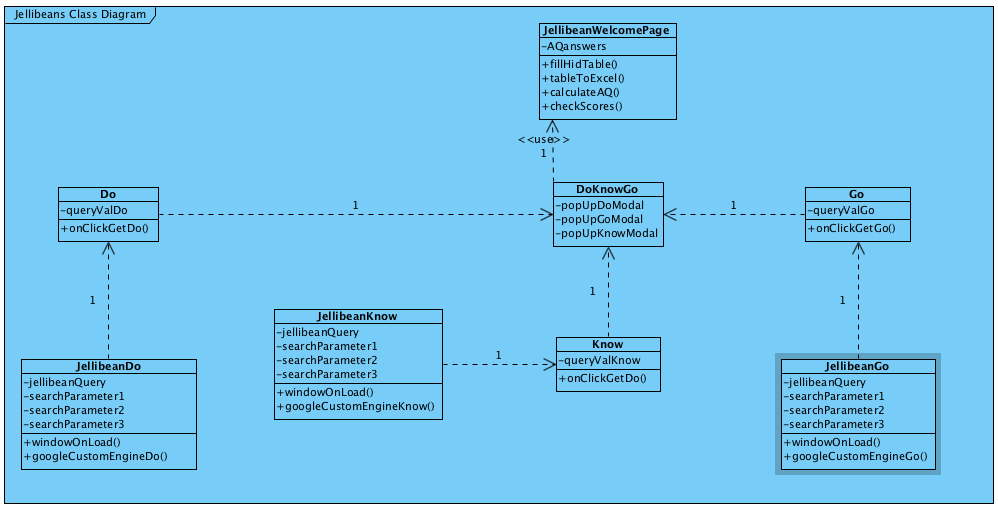
\includegraphics[scale=0.55]{jBeanClassDiagram}
\caption{High Level UML Class Diagram of Jellibeans.}
\end{center}
\end{figure}

\newpage
\subsection{Use Case Diagram}\label{JBeanUseCaseA}

\begin{figure}[H]
\begin{center}
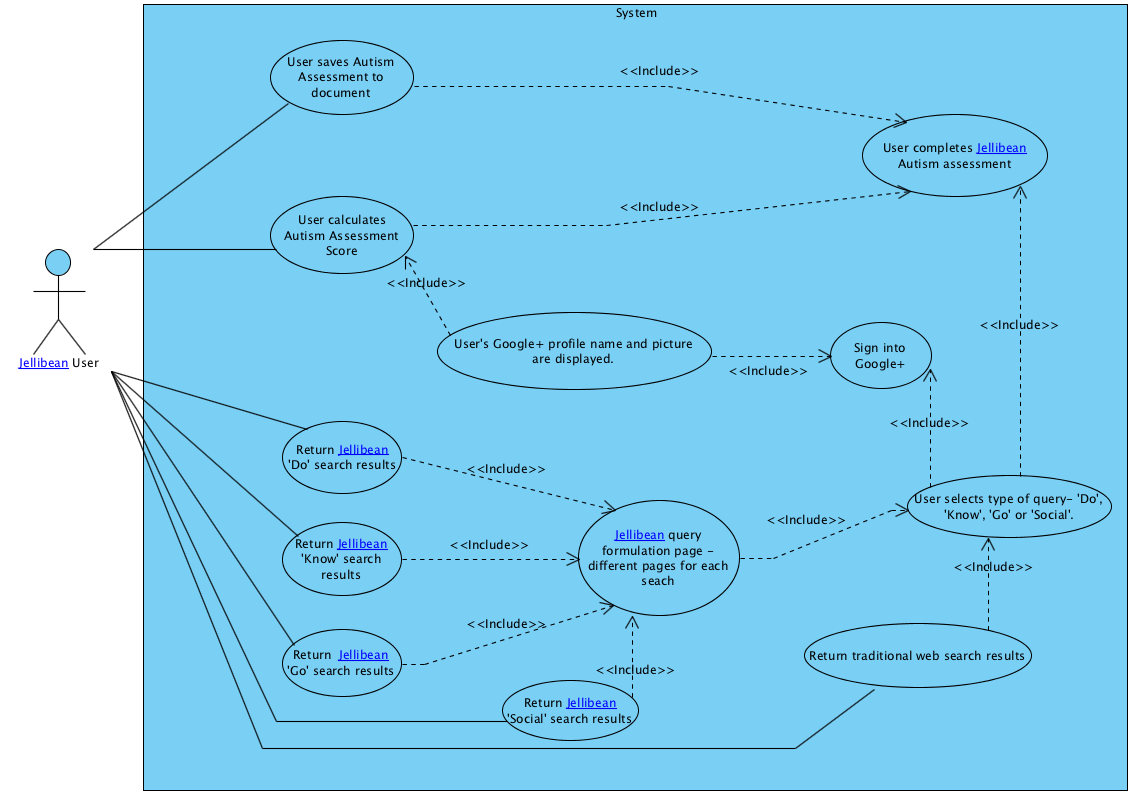
\includegraphics[scale=0.40]{JBeanUseCase}
\caption{Jellibean Feature Uses and High Level UML Use Case Diagram}
\label{JBeanUseCase}
\end{center}
\end{figure}


\newpage

\subsection{Languages and APIs Used in Jellibean Implementation}\label{implementation}

\begin{tabular}{l p{11cm} }
Google Search API & A RESTful API with a single method called list. The API method used was GET, and the response data is returned as a JSON type. The response consists of (1) the actual search result, (2) metadata for search like number of results, alternative search queries, and (3) custom search engine metadata. Google terms of service, state that `screen scraping', or copying the data directly from the website is prohibited.\\
JSoup API & For Bing and Yahoo search results, JSoup (a Java HTML parser) was used to identify the links from the resulting query. The JSoup HTML parser was considered more efficient for retrieving search results, as it could be used to complete the task from both search engines, using a slightly different href element filter for each. JSoup also has advantages over html parsing. It contains a class representing a list of nodes called `Elements', which implements Iterable to iterate over a list in an enhanced for loop.\\
Java & To test the combined output from the three search engines with a group of users, and gather their feedback on the results, I developed a Java Applet to run the programme. The search results from the Java Applet were written to a text file. Java was chosen for development of `to be tested' packages of features (e.g., the combination search engine). The developer for the project was most proficient with Java, and could quickly develop prototypes for user testing.\\
JavaScript & JavaScript is commonly used in HTML as it can run locally in a browser (rather than remote server). The Google+ API provided good documentation for using JavaScript. Furthermore the JavaScript code could be easily embedded into the Jellibean HTML code to interact with the Document Object Model (DOM) of the page. The browser was able to respond to user demand quickly, which made Jellibeans more responsive. JavaScript was used in this way to return the aboutMe profile information from Google+ to the user.\\
HTTP Set-Up & The Hypertext Transfer Protocol (HTTP) enables communications between web-browsers (clients) and the server (the computer that hosts Jellibeans) using a request-response protocol. Jellibeans was deployed in textbf{nginx} HTTP web server, and digitalocean.com was used to host the web servers, so that it was ready to be used remotely by users (and for me to gather feedback easily). When the user submits a HTTP request to the server that hosts Jellibeans, it responds with the appropriate behaviour to the client so that the user can formulate their search query and retrieve the results from their search. \\
JQuery & \\
php & \\

\end{tabular}

\begin{tabular}{l p{11cm} }
HTML & HyperText Markup Language (HTML 5) was used to create the webpages for Jellibeans, so that the web browser could render the wesite.\\
Bootstrap and CSS & For front-end development and to style the Jellibean web pages I used the Bootstrap framework \cite{bootstrap} for it's clear styles, good design and ease of use for the current project. I included my own Cascading Style Sheet (css file) where I needed extra styling beyond what the Bootstrap framework could offer. \\
LEAP SDK & The LEAP motion controller is a light-weight, portable device that detects user motions using infra-red light. The LEAP has accurate timing, and works well with the combinatorial configuration of senses (sight, hearing and touch). As this is a tool to be used with individuals with Autism, who have increased sensitivity to touch, the LEAP is the perfect choice as there is no additional sensations to the users body. The LEAP is affordable for users to integrate with search at home, and currently retails for about \pounds60.\\
LeapStrap & The LeapStrap SDK was used to integrate the LEAP into the web broswer. LeapStrap is a HTML5 front-end framework for websites, and gives them fill LEAP motion functionality. \\
\end{tabular}

\newpage
\subsection{Google Terms of Servive} \label{GoogleToS1}
\begin{figure}[H]
\begin{center}
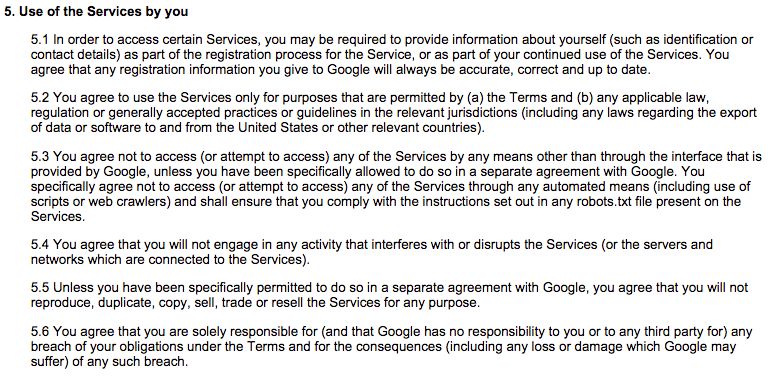
\includegraphics[scale=0.6]{GoogleToS}
\caption{Google Terms of Service}
\end{center}
\end{figure}

\newpage
\subsection{Search Query Survey} \label{AppendixA}

\begin{figure}[H]
\begin{center}
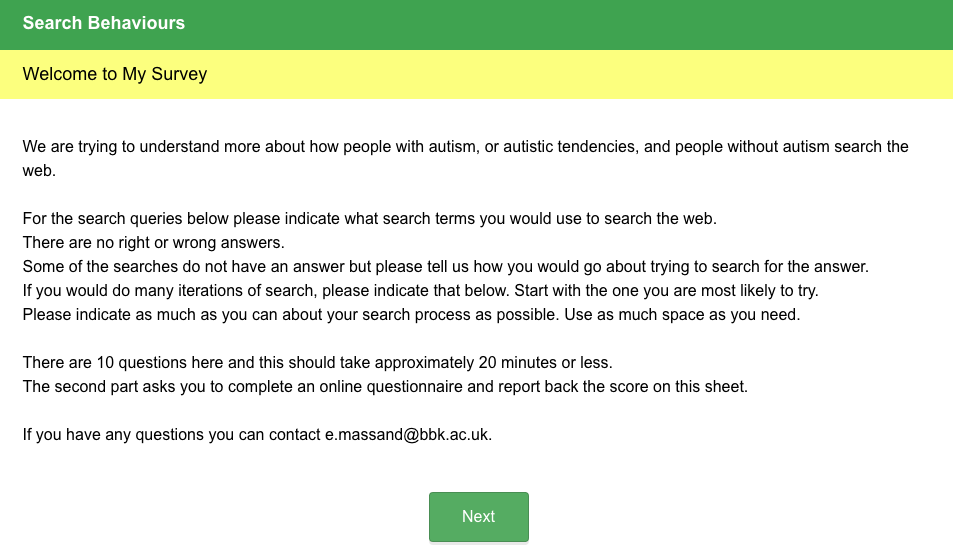
\includegraphics[scale=0.5]{survey1}\\
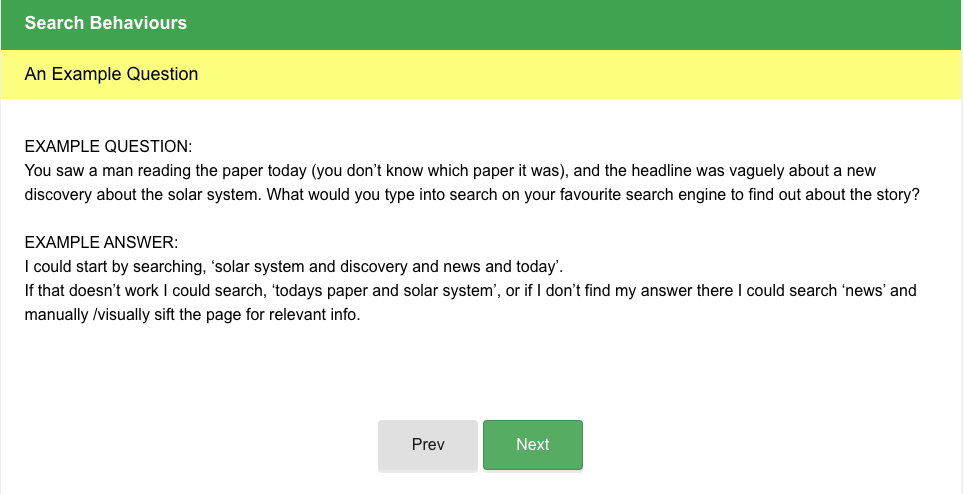
\includegraphics[scale=0.5]{survey2}\\
\end{center}
\end{figure}
\newpage
\begin{figure}[H]
\begin{center}
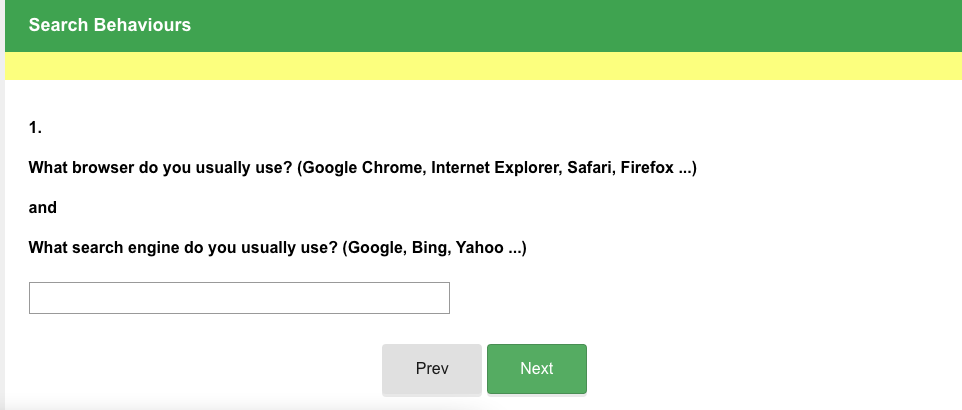
\includegraphics[scale=0.5]{survey3}\\
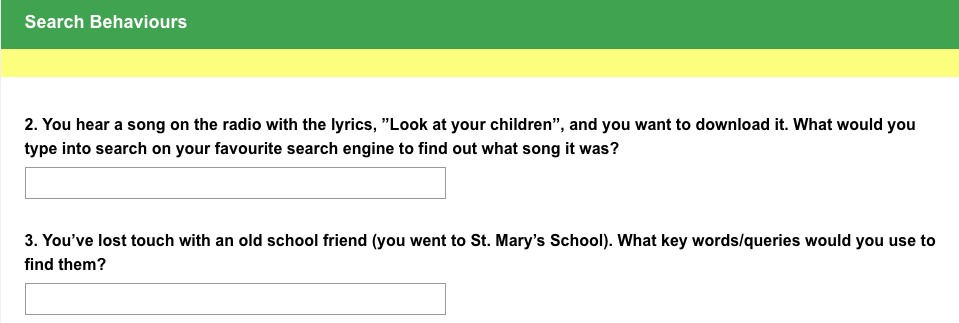
\includegraphics[scale=0.5]{survey4}\\
\end{center}
\end{figure}
\newpage
\begin{figure}[H]
\begin{center}
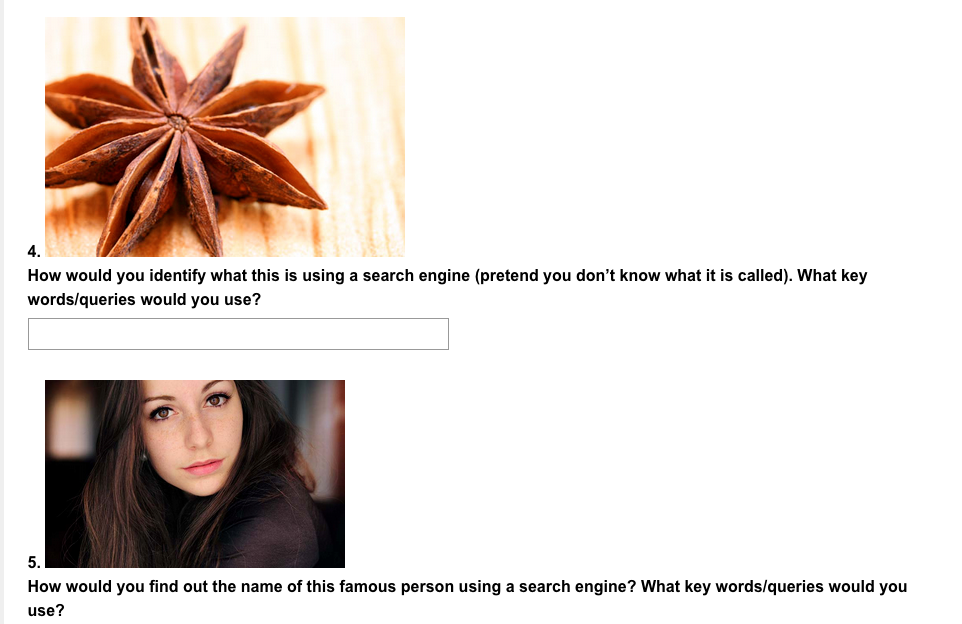
\includegraphics[scale=0.5]{survey5}\\
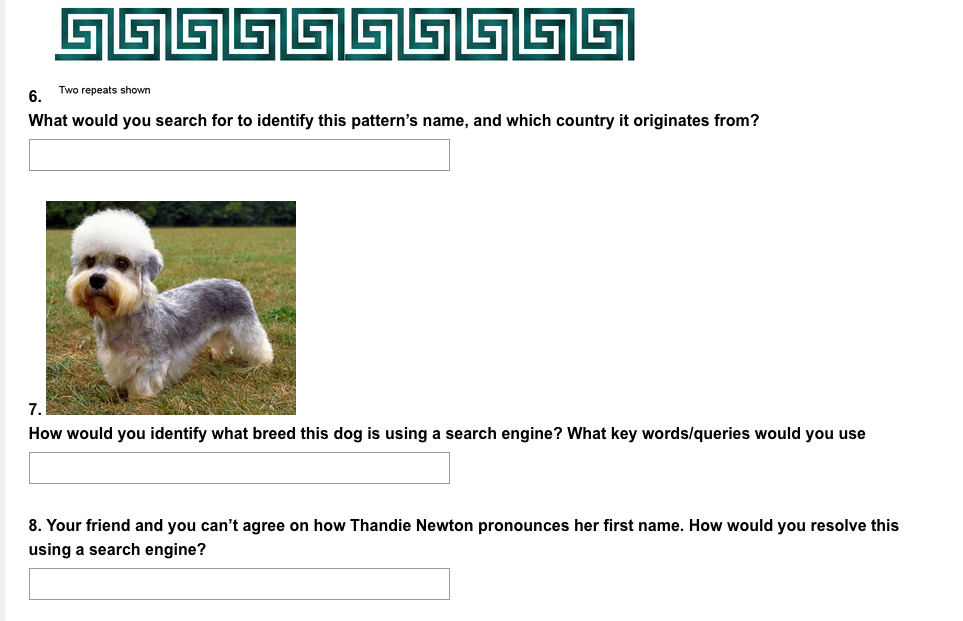
\includegraphics[scale=0.5]{survey6}\\
\end{center}
\end{figure}

\newpage
\begin{figure}[H]
\begin{center}
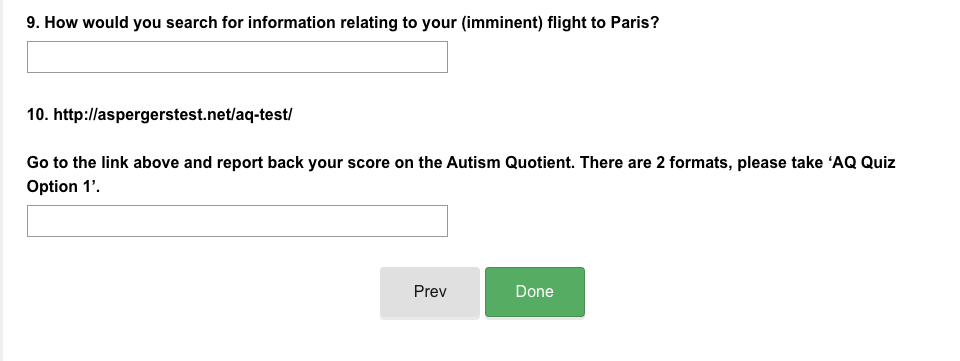
\includegraphics[scale=0.5]{survey7}\\
\caption{Search Query Survey on Surveymonkey.com \cite{surveymonkey}}
\end{center}
\end{figure}

\newpage
\subsection{Data Coding for Result 1 and 2}\label{datacoding}

\begin{figure}[H]
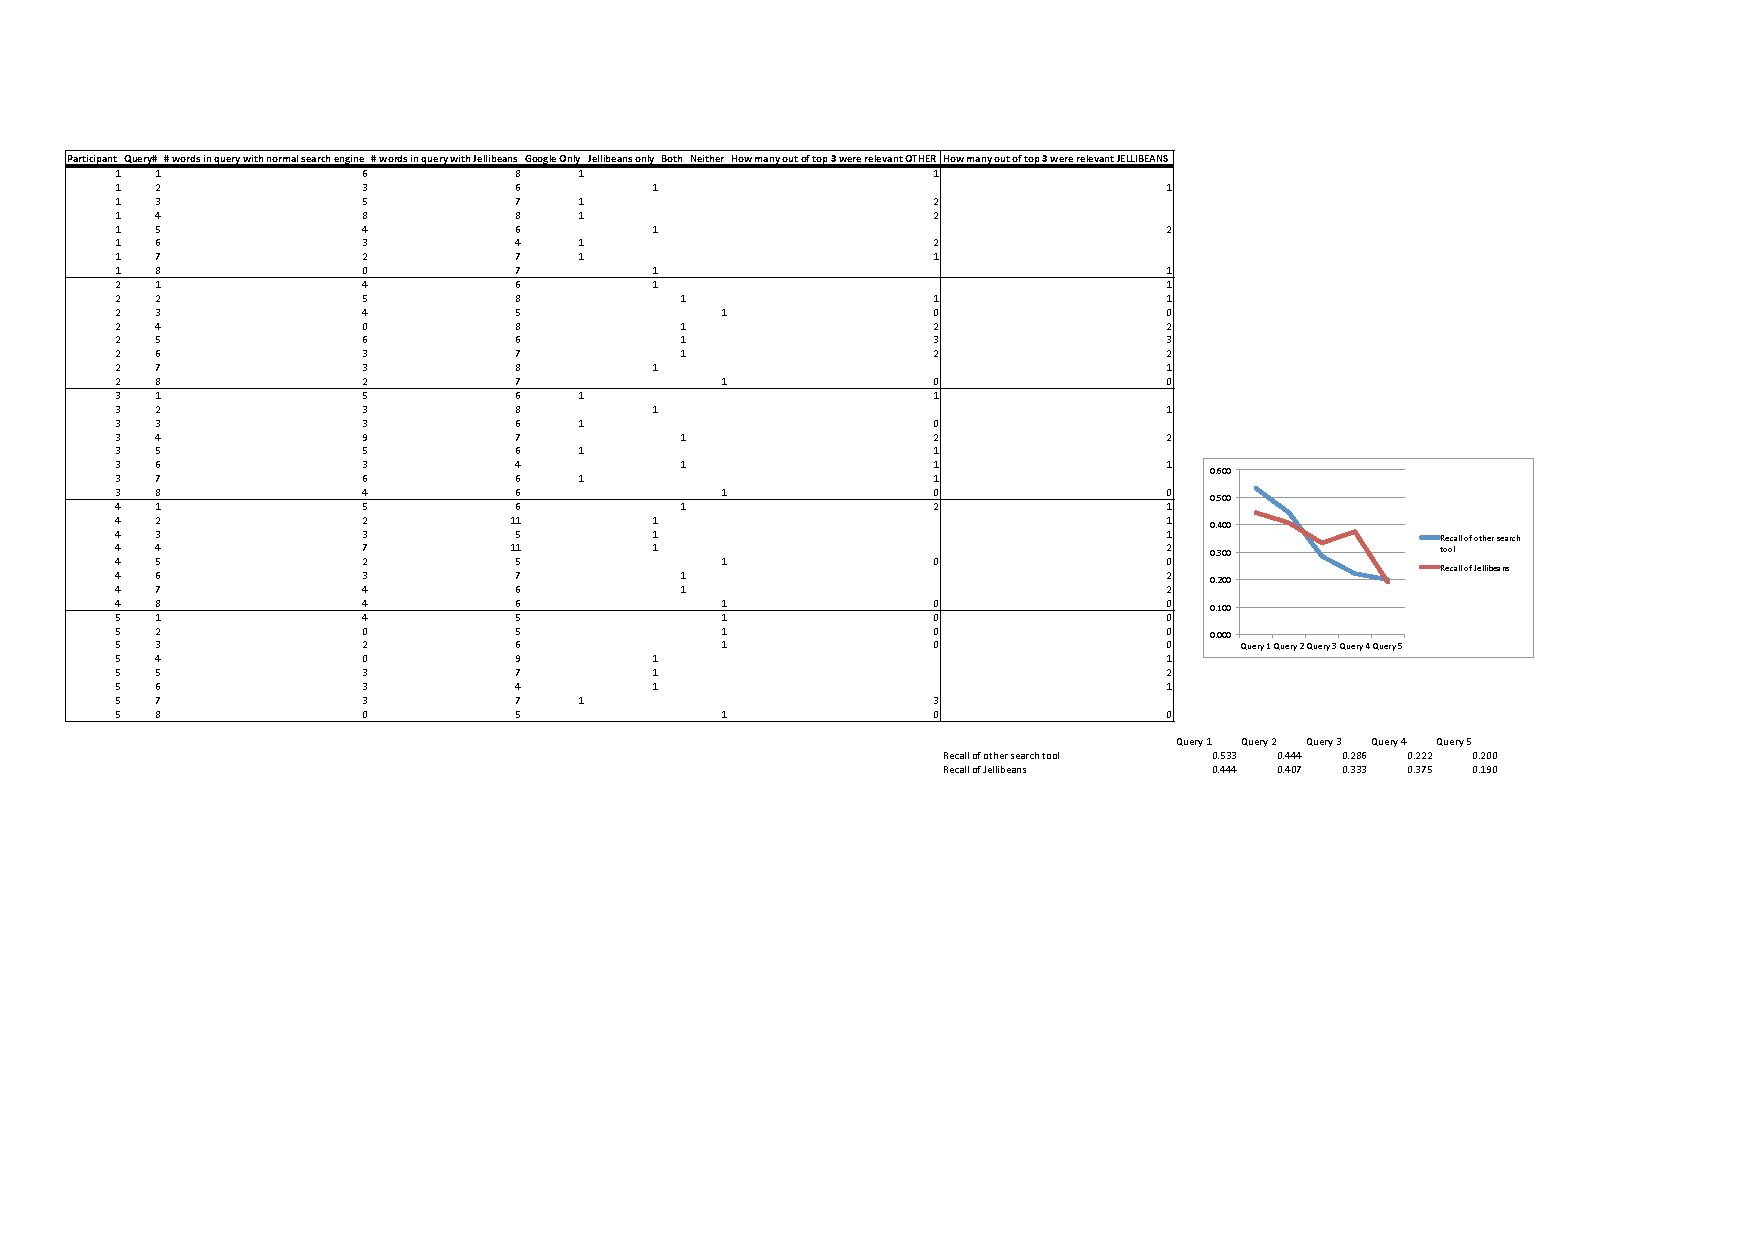
\includegraphics[angle=90, scale=0.57]{resultsCoding}\\
\caption{Data File for Results 1 and 2}

\end{figure}




\newpage
\subsection{Questions on the Autism Spectrum Quotient \cite{Baron Cohen et al}} \label{AQ}

Participants are asked to read each statement very carefully and rate how strongly they agree or disagree with the statement (Strongly Disagree, Slightly Disagree, Slightly Agree, or, Strongly Agree).  \\
\hspace{1cm}

I prefer to do things with others rather than on my own.\\
I prefer to do things the same way over and over again.\\
If I try to imagine something, I find it very easy to create a picture in my mind.\\
I frequently get so strongly absorbed in one thing that I lose sight of other things.\\
I often notice small sounds when others do not.\\
I usually notice car number plates or similar strings of information.\\
Other people frequently tell me that what I've said is impolite, even though I think it is polite.\\
When I'm reading a story, I can easily imagine what the characters might look like.\\
I am fascinated by dates.\\
In a social group, I can easily keep track of several different people's conversations.\\
I find social situations easy.\\
I tend to notice details that others do not.\\
I would rather go to a library than a party.\\
I find making up stories easy.\\
I find myself drawn more strongly to people than to things.\\
I tend to have very strong interests which I get upset about if I can't pursue.\\
I enjoy social chit-chat.\\
When I talk, it isn't always easy for others to get a word in edgeways.\\
I am fascinated by numbers.\\
When I'm reading a story, I find it difficult to work out the characters' intentions.\\
I don't particularly enjoy reading fiction.\\
I find it hard to make new friends.\\
I notice patterns in things all the time.\\
I would rather go to the theatre than a museum.\\
It does not upset me if my daily routine is disturbed.\\
I frequently find that I don't know how to keep a conversation going.\\
I find it easy to read between the lines when someone is talking to me.\\
I usually concentrate more on the whole picture, rather than the small details.\\
I am not very good at remembering phone numbers.\\
I don't usually notice small changes in a situation, or a person's appearance.\\
I know how to tell if someone listening to me is getting bored.\\
I find it easy to do more than one thing at once.\\
When I talk on the phone, I'm not sure when it's my turn to speak.\\
I enjoy doing things spontaneously.\\
I am often the last to understand the point of a joke.\\
I find it easy to work out what someone is thinking or feeling just by looking at their face.\\
If there is an interruption, I can switch back to what I was doing very quickly. \\
I am good at social chit-chat.\\
People often tell me that I keep going on and on about the same thing.\\
When I was young, I used to enjoy playing games involving pretending with other children.\\
I like to collect information about categories of things (e.g. types of car, types of bird, types of train, types of plant, etc.).\\
I find it difficult to imagine what it would be like to be someone else.\\
I like to plan any activities I participate in carefully.\\
I enjoy social occasions.\\
I find it difficult to work out people's intentions.\\
New situations make me anxious.\\
I enjoy meeting new people.\\
I am a good diplomat.\\
I am not very good at remembering people's date of birth.\\
I find it very easy to play games with children that involve pretending.\\

\end{document} 